% Chapter Template

\chapter{Introducción a la Superconductividad} % Main chapter title

\label{Chapter4} % Change X to a consecutive number; for referencing this chapter elsewhere, use \ref{ChapterX}

%----------------------------------------------------------------------------------------
%	SECTION 1
%----------------------------------------------------------------------------------------


El descubrimiento de que algunos materiales perdían su resistencia eléctrica a temperaturas muy bajas se realizó en 1911 y hasta 1986, las temperaturas críticas para todos los superconductores conocidos no superaron los 23 Kelvin ($23^{o}K$ o $-250^{o}C$). En 1986, se produjo un gran avance en la superconductividad cuando dos científicos, el Dr. K. Alex Muller y el Dr. J. Georg Bednorz, en un laboratorio de IBM en Zurich, Suiza, identificaron una cerámica. compuesto de óxido que se demostró que era superconductora a $36^{o}K$, ($-237^{o}C$). Este descubrimiento les valió el Premio Nobel de Física de 1987, (uno de los cuatro Premios Nobel que se han otorgado por trabajos en superconductividad). Posteriormente se descubrió una serie de compuestos de óxidos cerámicos relacionados que tienen temperaturas críticas más altas

Antes del descubrimiento y desarrollo de materiales de HTS (Alta Temperatura de Superconducción), el uso de la superconductividad no había sido práctico ni económico para aplicaciones comerciales, excepto para las aplicaciones de imágenes de resonancia magnética (MRI) y de almacenamiento de energía magnética superconductora (SMES), principalmente porque los superconductores disponibles comercialmente de LTS (Baja Temperatura de Superconducción) se hacen superconductores solo cerca del 0K. Aunque es tecnológicamente posible enfriar materiales LTS a una temperatura a la que se vuelven superconductores, la comercialización de materiales LTS no ha sido exitosa debido al alto costo asociado con el proceso de enfriamiento. Por ejemplo, el helio líquido, que se puede usar para enfriar materiales a aproximadamente $4^{o}K$ ($-269^{o}C$), y que se ha usado comúnmente para enfriar materiales LTS, es caro y sumamente costoso de mantener.

En la actualidad el superconductor HTS de mayor temperatura es el ${gBa_{2}Ca_{2}Cu_{3}O_{8}}$ o más sintéticamente $Hg-1223$, de estructura cristalina tetragonal y de temperatura de superconductividad de $134^{o}K$ ($-139^{o}C$) temperatura fácilmente alcanzable con aire líquido (punto de fusión: $-216.2^{o}C$, punto de ebullición: $-194.35^{o}C$)


\section{Conductividad clásica}
\label{sec:pruebasHW}

\subsection{Resistencia residual} 

Un electrón libre puede moverse en un cristal perfecto sin pérdidas de energía. cualquier irregularidad en la estructura genera dispersión en los electrones produciendo una resistencia. Aún a $0^{o}K$ hay una variedad de defectos que generan resistencia eléctrica.

La discrepancia entre los valores calculados teóricamente y los medidos experimentalmente debe a que la estructura cristalina real difiere de la ideal, de esta manera aparecen dos resistividades: una térmica ($\rho_{T}$) y otra residual ($\rho_{R}$) la segunda es ocasionada por defecto reticulares. el trabajado en frío del metal agrega otro término que es determinado experimentalmente. La resistividad aumenta linealmente con la temperatura:


\begin{equation}
\rho(T)= \rho_{0}(1+\alpha \delta T) = \rho_{R} + \rho_{T} \quad \text{\textbf{Regla de G\"uneisen}}  
\end{equation}

Para la mayoría de los metales puros a excepción de los de transición $\alpha$ vale aproximadamente $4,0.10^{-3}$, los de transición y en particular lo ferrosos tienen valores más altos: $\alpha \approx 10^{-2}$

Para temperaturas muy bajas se demuestra que la resistividad es proporcional a $T^{5}$ .

\begin{equation}
	\rho(T)= \rho_{0}+\alpha T^{5} \quad \text{\textbf{Regla de Mathiessen}}  
\end{equation}

La medición experimental de la resistividad es un método cómodo Y preciso para determinar indirectamente propiedades de los metales y aleaciones, tales como transformaciones envejecimiento, transformaciones magnéticas etc, usando un alambre de platino puede confeccionarse un termómetro patrón. Existe una gran cantidad de trabajo sobre la resistividad de aleaciones y otras propiedades, por ejemplo: variación de la resistividad con el endurecimiento del metal, daño por radiación, etc.

\subsection{Conductividad y aleaciones}

Los aleantes, invariablemente aumentan la resistividad. Este efecto es diferente en los semiconductores. En el esquema se observa Cómo varía la resistividad del cobre con el agregado de una impureza en función de la temperatura. La dependencia de la resistividad residual ($\rho_{R}$) en el caso de un solo tipo de impureza está dada por:

\begin{equation}
\rho_{R}=AX(1-X) \quad \text{\textbf{Regla de Nordheim}}
\end{equation}

Donde $S$ es la concentración y $A$ es una constante que depende del solvente si $X \ll A$, solución diluida, entonces:
\[
\rho_{R} \approx AX 
\]

El aumento lineal de la resistividad depende de $\rho_{R}$ ya que $\rho_{T}$ permanece constante.

\begin{figure}[H]
    \centering
    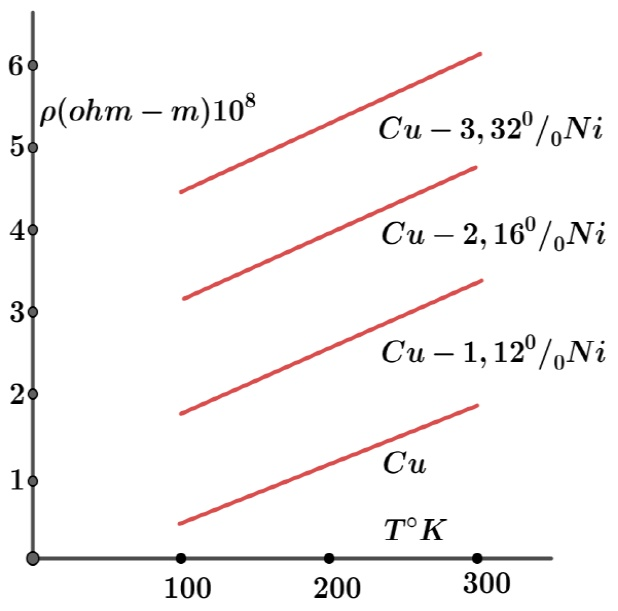
\includegraphics[width=0.5\textwidth]{./Figures/fig42}
	\caption{$\rho$ del $Cu$ para distintas concentraciones de $Ni$}
	\label{fig:42}
\end{figure}

\subsubsection{Conductividad y trabajo mecánico}

En el esquema de la figura \ref{fig:44} se puede observar la curva de un recocido anisotérmico para níquel trabajado en frio, se ve la curva correspondiente a la recuperación y recristalización del material (curva en azul),también se trazaron la dureza (negro) y densidad (rojo), donde queda de manifiesto la importancia del trabajado mecánico y restauración del material sobre la resistividad del mismo. Vemos que el cambio fundamental en la dureza ocurre simultáneamente con la recristalización de la matriz. Se comprueba que el aporte de las dislocaciones es muy pequeño comparado con lo que aportan los defectos puntuales.

\begin{figure}[H]
    \centering
    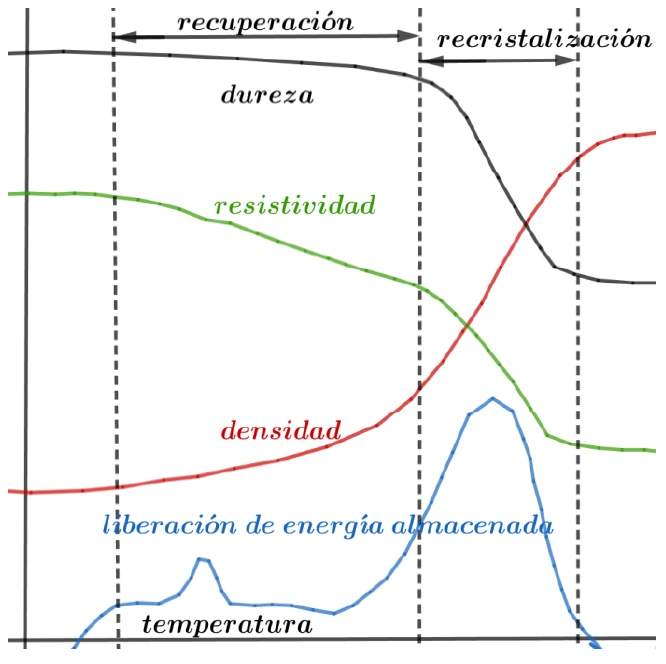
\includegraphics[width=0.5\textwidth]{./Figures/fig43}
	\caption{Recocido anisotérmico para $Ni$}
	\label{fig:44}
\end{figure}


\subsubsection{Aleaciones para conductores y aisladores}

De lo estudiado previamente se infiere que los materiales para conductores deben ser fabricados con metales lo más puro posibles. Por otro lado, los materiales para resistencia necesariamente deben ser aleaciones (soluciones sólidas).

$\centerdot$ \textbf{Conductores:}
Los metales más usados para conductores son el $Cu$ y el $Al$. Con el fin de aumentar su resistencia mecánica en el caso del $Cu$ se introducen impurezas de $Cd$, $Sn$, $Al$, $P$, $Cr$, $Be$, por supuesto que disminuyendo la conductividad eléctrica. La aleación más difundida es $Cu-0,9Cd$, cuya conductividad es de hasta 90\% de la del cobre. La conductividad eléctrica del aluminio es un 65\% de la del $C$u, con el fin de aumentar la resistencia mecánica se agrega magnesio y silicio. Véase la figura \ref{fig:46}

\begin{figure}[H]
    \centering
    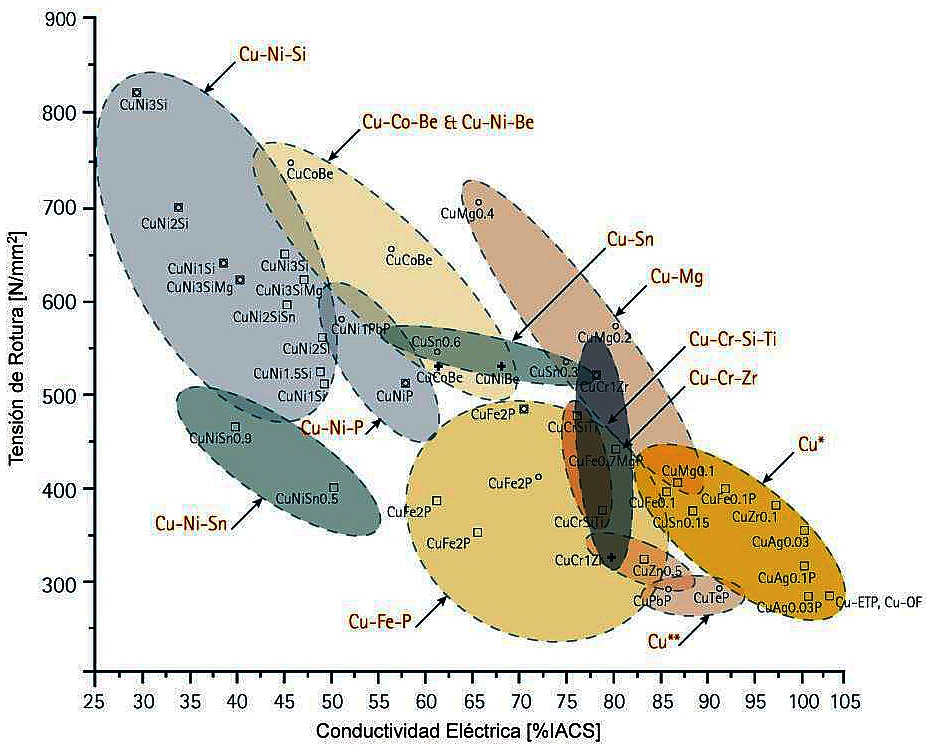
\includegraphics[width=0.9\textwidth]{./Figures/fig46}
	\caption{Conductividad y tensión de rotura}
	\label{fig:46}
\end{figure}

En la figura \ref{fig:47} Podemos ver cómo influye cada elemento agregado al $Cu$ en su conductividad total. El más favorecedor es la Plata, seguido por el Oxigeno. Cuando el Cobre no será sometido a esfuerzos mecánicos, de alea libre de Oxígeno constituyendo lo que se conoce como cobre libre de oxígeno (OFC) o el cobre libre de oxígeno de alta conductividad térmica (OFHC); un grupo de aleaciones de cobre forjado de alta conductividad que se han refinado electrolíticamente para reducir el nivel de oxígeno a 0,001\% o menos.

\begin{figure}[H]
    \centering
    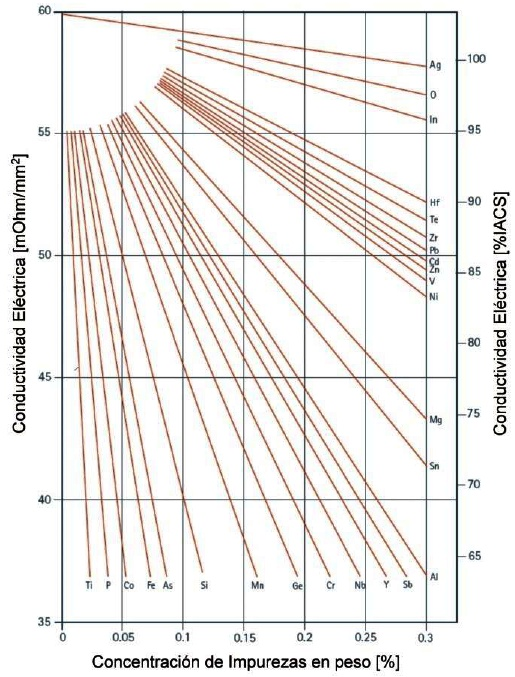
\includegraphics[width=0.8\textwidth]{./Figures/fig47}
	\caption{Conductividad y concentración de impurezas}
	\label{fig:47}
\end{figure}


$\centerdot$ \textbf{Resistores:}
En estos casos se requiere alta resistencia eléctrica y pequeño coeficiente de temperatura y refractarias, por tanto, generalmente se usan aleaciones de hierro con impurezas que forman soluciones solidas. El carácter refractario esta dado por el agregado de cromo y aluminio.


\section{Superconductividad}

En un comienzo se pensó que era un fenómeno particular de algunos metales, hoy, el número de aleaciones, elementos y compuestos con propiedades superconductoras es enorme y nos deberíamos preguntar ¿cuales sustancias no son superconductoras?.

La superconductividad ofrece una oportunidad única para observar fenómenos cuánticos macroscópicos. La razón de esto es que los circuitos superconductores cerrados (como se verá) solo pueden contener unidades discretas de flujo magnético.

Es una de las áreas más atractivas y particulares de la física.

La superconductividad fue observada por primera vez en 1911 por Gilles Holst quien trabajaba en el laboratorio de Kamerlingh Onnes, el mismo que tres años antes en 1908 habia obtenido la licuefacción del Helio. El notó que la resistividad del mercurio se anulaba de repente debajo de los 4,2 Kelvin. Este fenómeno recibe el nombre de superconductividad. Cómo fue visto sabemos que la resistencia eléctrica se debe a que los electrones que forman la corriente sufren colisiones con las impurezas y defectos de la estructura cristalina, la energía cinética de los electrones se pierde en forma de calor. La teoría de la conducción eléctrica en los metales establece que si la muestra no tiene defectos impurezas resistividad debería tender a cero cuando $T\rightarrow 0$. Sin embargo existe un amplio número de sustancias, metales, aleaciones, compuestos intermetalicos, etc cuya resistencia desciende a cero antes del cero grado Kelvin. La temperatura a la cual se hace 0 a la resistencia eléctrica de una sustancia llama temperatura crítica $T_{c}$. Entre los elementos puros se pueden encontrar más de 30 superconductores. La superconductividad no es un fenómeno clásico, normalmente se trata a los electrones en un metal como un gas de Fermi, la superconductividad difiere de este caso y es una consecuencia esencialmente mecánico cuántico de las interacciones entre electrones las cuales se ignoran en el modelo de partículas libres. \textbf{Lo interesante de estos materiales es que nos permite observar fenómenos cuánticos a muestro nivel, sin microscopio}.

\begin{figure}[H]
    \centering
    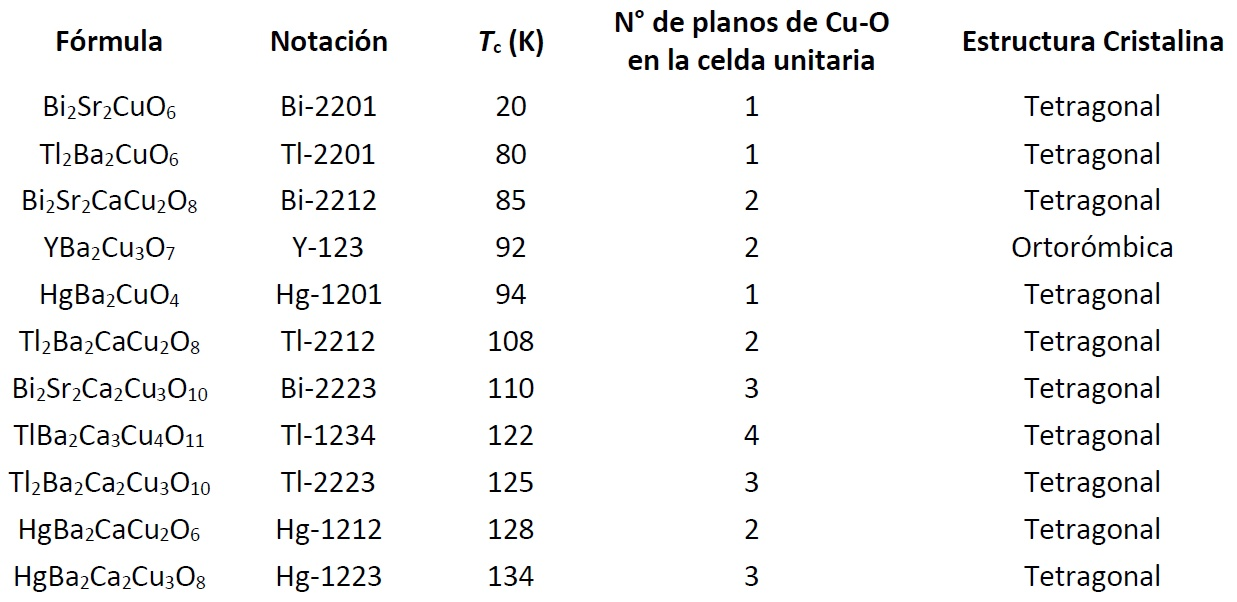
\includegraphics[width=1.0\textwidth]{./Figures/fig48}
	\caption{Diversos superconductores cerámicos}
	\label{fig:48}
\end{figure}



\begin{figure}[H]
  \begin{minipage}[b]{0.47\textwidth}
En el esquema se observan los resultados obtenidos por Onnes. Si $T<T_{c}$ la resistencia del conductor es cero. Notablemente, los buenos conductores a temperatura ambiente como el cobre y la plata no presentan superconductividad. Tampoco la mayoría de los metales ferromagnéticos. La temperatura crítica depende de la ubicación del elemento en la tabla periódica. Desde que se descubrió la superconductividad hasta las primeras explicaciones del fenómeno pasarán más de 50 años.
  \vspace{0.0cm}
  \end{minipage}
  \hfill
  \begin{minipage}[b]{0.47\textwidth}
     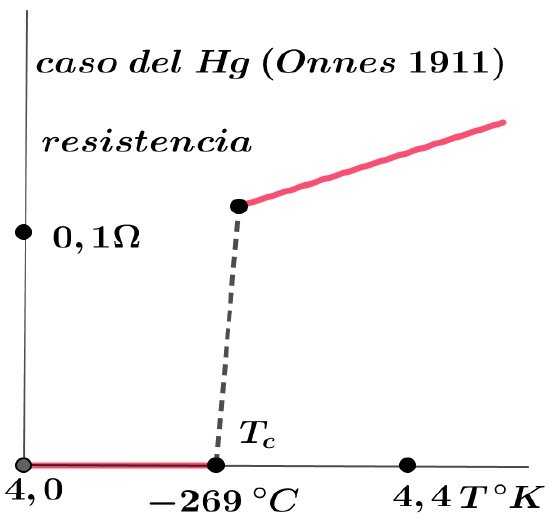
\includegraphics[width=0.9\textwidth]{./Figures/fig44}
     \caption{Superconductividad del $Hg$}
	\label{fig:44}
	  \vspace{0.0cm}
  \end{minipage}
\end{figure}

En la figura \ref{fig:45} vemos en el caso general el comportamiento a bajas temperaturas de un material normal y un superconductor.

\begin{figure}[H]
    \centering
    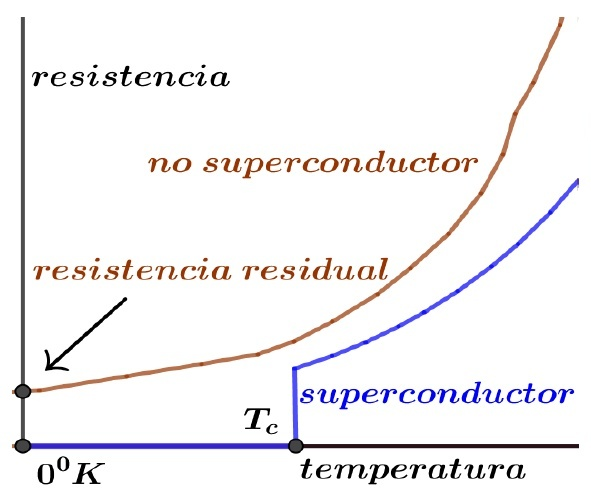
\includegraphics[width=0.5\textwidth]{./Figures/fig45}
	\caption{Comportamientos a bajas temperaturas}
	\label{fig:45}
\end{figure}
	



\subsection{Propiedades de la superconductividad}

Se ha observado experimentalmente que:

\begin{itemize}
	\item Si por un anillo superconductor se hace pasar una corriente, ésta se ha conservado por más de 2 años.
	
	\item Aunque existan cantidades importantes de impurezas en una sustancia no modifica la temperatura crítica tal como vemos en la figura \ref{fig:49}
	
	
\begin{figure}[H]
    \centering
    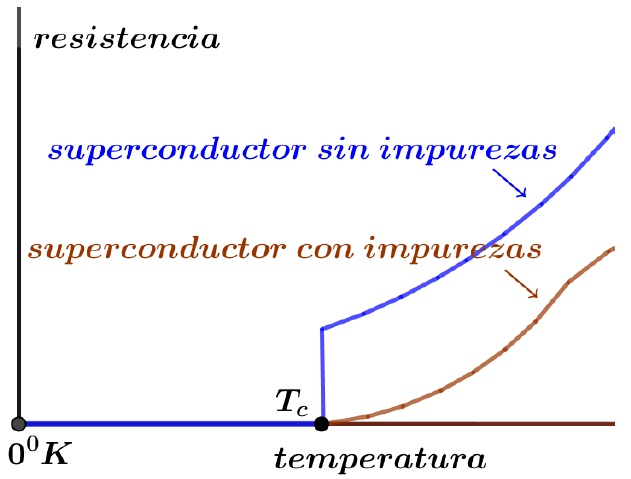
\includegraphics[width=0.6\textwidth]{./Figures/fig49}
	\caption{Efecto de las impurezas}
	\label{fig:49}
\end{figure}
	
	
	
	\item Podría pensarse que el paso a la superconductividad se debe algún cambio en la estructura cristalina del metal. Sin embargo distintos estudios dieron resultados negativos se sabe que los electrones libres en un metal aportan el calor específico a temperatura ambiente este aporte es despreciable contrario a bajas temperaturas el calor específico debido a las
vibraciones de la red decrece cubicamente, mientras que la debida al gas de electrones lo hace linealmente. La dependencia del calor específico de un metal no superconductor en la zona de bajas temperaturas tiene la expresión siguiente:

\begin{equation}
	C= AT^{2}+BT
\end{equation}

el primer término es debido a la red y el segundo a los electrones. El aporte de la estructura (vibración de la red) al calor específico en un superconductor sigue siendo el mismo, que en un material normal, esto indica que no hay calor latente durante la transformación. Lo que significa que la transición a la superconductividad es una transformación de segundo orden, el calor específico no es discontinuo. Necesariamente los cambios se deben al calor específico de los electrones que responde a la siguiente expresión

\begin{equation}
	C= AT^{3}+De^{-\mfrac{b}{kT}}
\end{equation}

	\item Probetas hechas con isótopos de un mismo elemento poseen temperaturas críticas diferentes. Este resultado muestra que sí bien la estructura cristalina no se modifica al pasar al estado superconductor, si desempeña un papel importante en la variación de las propiedades del gas electrónico (interacción de los electrones con las vibraciones de la red).
	
	\item La temperatura crítica depende de la masa isotropica ($M$) a través de la siguiente expresión:
	
\begin{equation}
	M^{\alpha}= const
\end{equation}
	
	\item No habría ninguna razón para pensar que $T_{c}$ dependa de número de neutrones del material salvo por el hecho, que las vibraciones de la red si dependen de la masa del núcleo atómico.
	
	\item La dependencia del calor específico con la temperatura,sigue una relación como la ilustrada en la figura \ref{fig:410}, lo cual indica que estamos frente a una transformación de segundo orden
	
\begin{figure}[H]
    \centering
    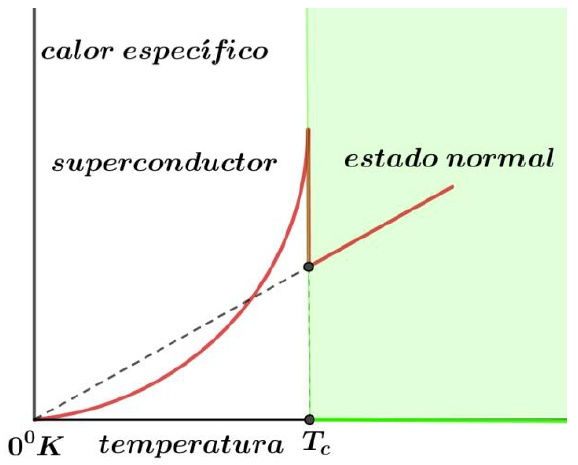
\includegraphics[width=0.5\textwidth]{./Figures/fig410}
	\caption{Transformación de segundo orden en el calor específico}
	\label{fig:410}
\end{figure}
	
	\item Se esperaba que la superconductividad poder crear campos magnéticos intensos sin disipación, pero se comprobó que campos magnéticos muy intensos hacen desaparecer la superconductividad. El campo magnético al cual desaparece la superconductividad se lo llama campo crítico $H_{c}$. Luego se vio que existe una relación entre la temperatura crítica y el campo crítico $H_{c}=f(T_{c})$. En estados donde el campo $H$ es mayor que el crítico $H_{c}$ no se logra superconductividad nunca.	
	
	\item En el esquema de la figura \ref{fig:411} se observa la variación del campo crítico en función de la temperatura crítica. Este gráfico nos muestra que la transición de estado normal a superconductividad es reversible. Para un campo y temperatura dados, existe un estado de equilibrio único que puede ser interpretado como una curva de transición de fase y por tanto puede ser aplicada a la termodinámica. En ausencia de campo magnético vimos que la transiciones de segundo orden cuando existe un campo magnético externo es de primer orden (esto se verá ampliado cuando tratemos el calor latente de la transformación).	
	
\begin{figure}[H]
    \centering
    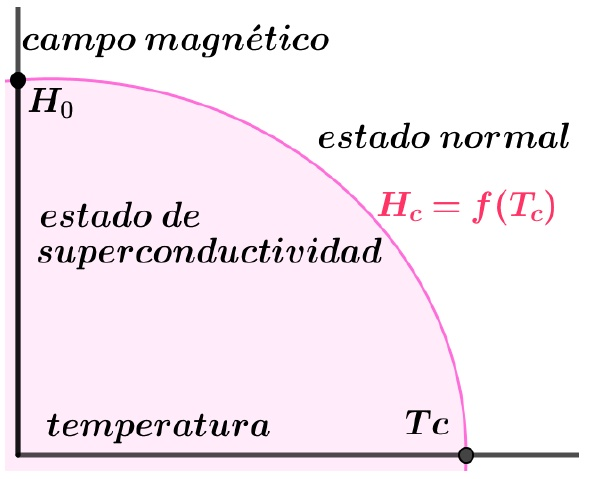
\includegraphics[width=0.5\textwidth]{./Figures/fig411}
	\caption{Superconductividad y estado normal}
	\label{fig:411}
\end{figure}

Observamos que la curva  $H_{c}=f(T_{c})$ divide al plano $H,T$ en dos regiones: superconductor y normal, de manera similar a una curva de cambio de fase en un diagrama $p,T$ . La mayoría de los superconductores cumplen con la siguiente expresión que nos da el campo crítico en función de la temperatura:	
	
\begin{equation}
	 H_{c}=f(T_{c}) = H_{0}\big( 1- \mfrac{T^{2}}{T_{c}^{2}}    \big)
\end{equation}
	
\end{itemize}


\begin{figure}[H]
    \centering
    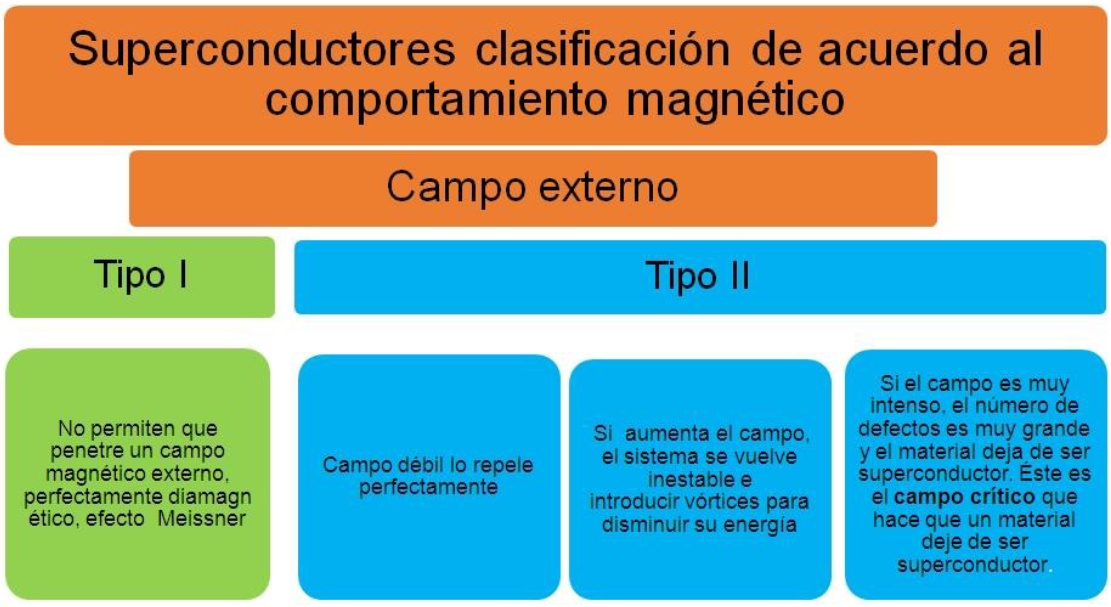
\includegraphics[width=1.0\textwidth]{./Figures/fig412}
    \caption{Características Superconductores tipo I y II}
	\label{fig:412}
\end{figure}


\subsection{Superconductores tipo I}

El Efecto Meissner consiste en la desaparición total del campo magnético constante en el interior de un superconductor desafiado por debajo de su temperatura crítica las líneas de inducción B son zonas del interior del cuerpo. Por tanto el material se comporta como un diamagnético perfecto con susceptibilidades muy superiores a las de los materiales diamagnéticos estándar puesto que no permite que ingrese en él un campo.

\begin{equation}
	B=0 \; \text{como}  \; B=\mu_{0}(M+H) \; \text{entonces}  \; M=-H  \; \text{luego}  \; \chi=\mfrac{M}{H} = -1  \; \text{en el sistema SI} 
\end{equation}

Un material superconductor tipo 1 es perfectamente diamagnético en la figura \ref{413} está representado este comportamiento:


\begin{figure}[H]
    \centering
    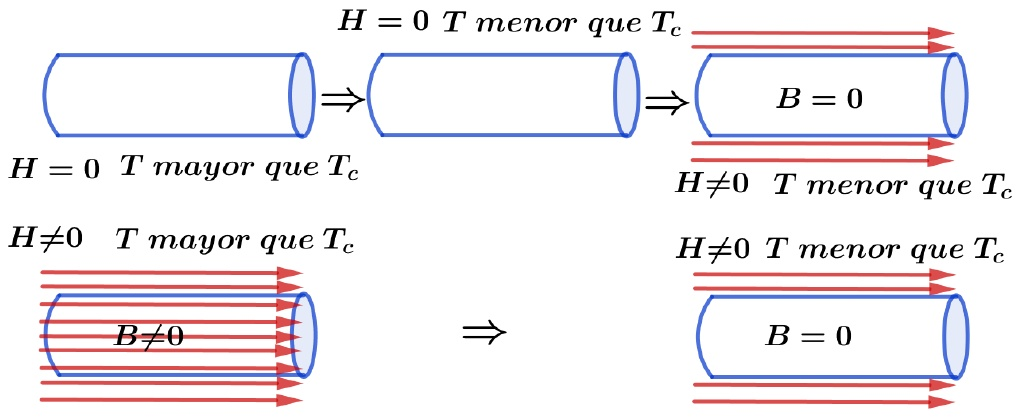
\includegraphics[width=0.9\textwidth]{./Figures/fig413}
    \caption{Superconductor tipo I}
	\label{fig:413}
\end{figure}

Este comportamiento singular se debe macroscópicamente a la circulación de una corriente cerca de la superficie del material, llamada supercorriente , o corriente persistente que da lugar a un campo magnética interno igual y opuesto al externo, creando una pantalla magnética.


\begin{figure}[H]
  \begin{minipage}[b]{0.47\textwidth}
Efecto Meissner: un magneto levitando sobre un superconductor (enfriado por nitrógeno líquido)
  \vspace{1.0cm}
  \end{minipage}
  \hfill
  \begin{minipage}[b]{0.47\textwidth}
     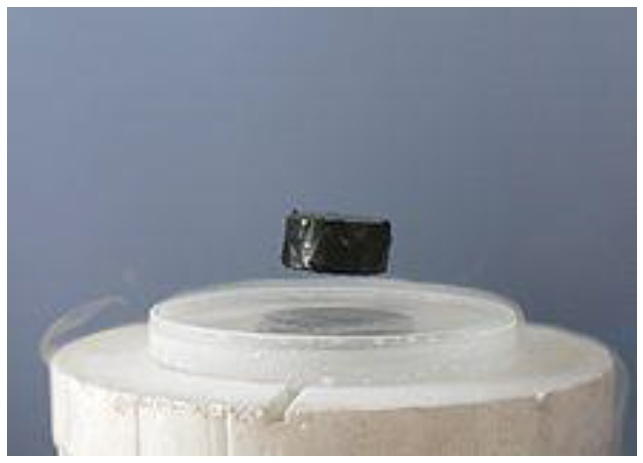
\includegraphics[width=0.9\textwidth]{./Figures/fig414}
	\label{fig:44}
	  \vspace{0.0cm}
  \end{minipage}
\end{figure}


\begin{figure}[H]
  \begin{minipage}[b]{0.47\textwidth}
     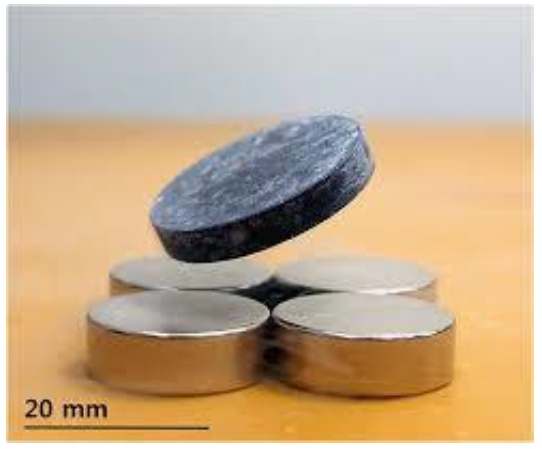
\includegraphics[width=0.9\textwidth]{./Figures/fig415}
	\label{fig:415}
	  \vspace{0.0cm}
  \end{minipage}
   \hfill
  \begin{minipage}[b]{0.47\textwidth}
Efecto Meissner: un superconductor (previamente enfriado por nitrógeno líquido) levitando sobre un grupo de magnetos
  \vspace{1.0cm}
  \end{minipage}
\end{figure}


\subsection{Conductor Perfecto}

En este punto desarrollo, uno se podría preguntar: ¿es un superconductor un conductor perfecto?. La respuesta es ¡!no!!. Por supuesto, hay muchas similitudes entre los dos conceptos, principalmente porque ambos son tipos de conductores especiales, pero hay una clara delimitación en lo que respecta a sus principios operativos. Los superconductores realmente existen, pero un conductor perfecto es un concepto, asumido por los físicos. En realidad, no hay nada como un conductor perfecto, de la misma manera que no hay nada como un gas ideal. Los conductores perfectos son perfectos a cualquier temperatura, los superconductores sólo existen por debajo de la temperatura crítica del material. Estudiemos Qué sucede con el campo magnético en distintos casos.

¿Qué pasaría si el conductor es real?, supongamos un conductor que introducimos en un campo magnético y por lo tanto en un flujo $\phi$

\begin{equation}
	\varphi=\oiint_{Sup}\V{B} \cdot d\V{s } \, \text{y por la ley de Lenz se genera una fem} \; \varepsilon=\frac{d\phi}{dt}
\end{equation}

Creando una corriente $i$I que genera un campo que se opone al cambio del campo original, luego:

\begin{equation}
	- \varepsilon= Ri+L\frac{di}{dt}
\end{equation}

Con $R$ y $L$ representamos la resistencia y la inductancia del circuito. Resolviendo la ecuación diferencial a que la corriente inducida se extingue con una constante de tiempo $\tau=\frac{R}{L}$ cuando menor es $R$ más rápidamente se alcanzará el estado estacionario.

Entendemos por conductor perfecto, un material que obedece a la ley de Ohm pero con resistencia despreciable. Suponemos un conductor perfecto por el que circula una densidad de corriente finita J , y puesto que cumple con la ley de Ohm: $\V{J}=\sigma \V{E}$

Como el conductor es perfecto cuando $\sigma\rightarrow \infty$ Entonces el campo $\overrightarrow{E}$ tiende a 0 pues, de lo contrario la densidad de corriente sería infinita. Por la ley de Faraday:

\begin{equation}
	\nabla \times \V{E}= -\frac{d\V{B}}{dt} = 0 \rightarrow \V{B} = Ctte
\end{equation}

En el interior de un conductor perfecto $\V{B} = Ctte$ Veamos en qué se diferencia un conductor perfecto de un superconductor.

\subsubsection{Enfriamiento con y sin campo B}

En un primer caso enfriamos el material sin la presencia de campo magnético. Tenemos el material a muy baja temperatura, y colocamos un campo externo, el campo no puede ingresar al metal ya que la variación del campo (por la ley de Lenz) genera corriente que se opone a que ingrese (si el campo en un comienzo fue cero debe seguir siendo cero). Por otro lado, si tenemos un campo $\V{B}$ en el interior del conductor y enfriamos, no puede dejar de estar este campo. Esto se observa en la figura \ref{fig:416}:

\begin{figure}[H]
    \centering
    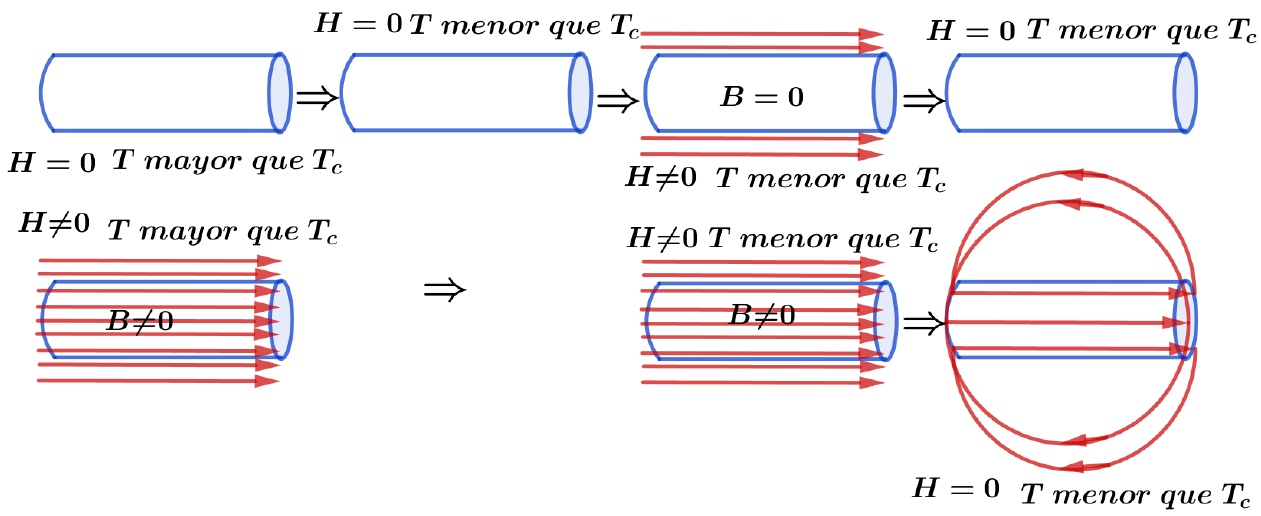
\includegraphics[width=1.0\textwidth]{./Figures/fig416}
    \caption{Conductor perfecto y superconductor 1}
	\label{fig:416}
\end{figure}

Luego vemos que los superconductores son algo más que materiales con conductividad perfecta, tienen algo más que un conductor perfecto. Un superconductor tipo I nunca deja que exista un campo en si interior. Dicho de otro modo, su característica principal es que son diamagnéticos perfectos. Observemos que el comportamiento de un superconductor no depende de la historia, si el conductor perfecto.

\subsection{Superconductor y conductor perfecto}

Un material en el estado superconductor tiene dentro $B=0$ independientemente de si el campo magnético externo se aplicaba antes o después del enfriamiento por debajo de la temperatura crítica. Este efecto de expulsión del campo magnético externo distingue a un material superconductor de un material perfectamente conductor y toma el nombre de efecto Meissner.

Las corrientes de protección o apantallamiento de la superficie también están presentes en un conductor perfecto y explican la falta de penetración en el material del campo magnético aplicado después del enfriamiento, véase la figura \ref{fig:417}. 

\begin{figure}[H]
    \centering
    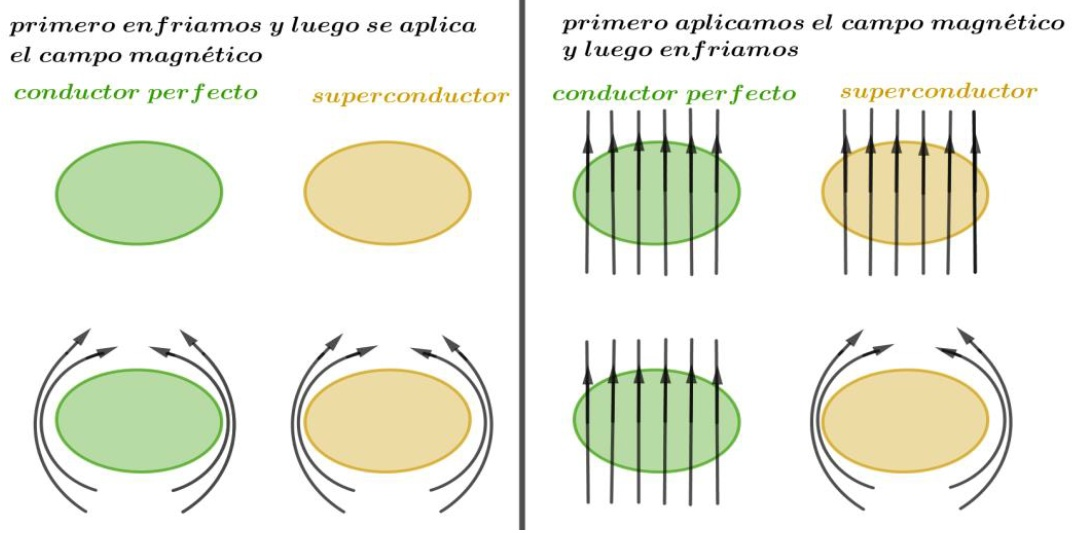
\includegraphics[width=1.0\textwidth]{./Figures/fig417}
    \caption{Conductor perfecto y superconductor 2}
	\label{fig:417}
\end{figure}

\subsubsection{Preguntas}

\begin{itemize}
	\item Razonando sobre el esquema de los cilindros superconductores, vimos que en cualquiera de los dos casos; colocando el campo antes o después de enfriar el campo es cero ($B=0$) en el superconductor. La explicación por la aparición de una súper corriente que anula el campo aplicado en el interior del metal. Si ahora anulamos el campo aplicado siempre a ($T<T_{c}$) la súper corriente tendría que oponerse a esta modificación y Eternamente tendríamos un campo y una corriente en el superconductor, ¿es correcto?.
	
	\item Pasemos el diagrama del conductor perfecto. Vimos que un conductor real tarda un tiempo igual a $\tau=R/L$ para extinguir la corriente inducida, ¿En un conductor perfecto tardaría un tiempo infinito en desaparecer?. ¿Luego, nunca se extinguiría? y ¿Cuánto tiempo tardaría en establecerse la corriente de apantallamiento?
	
	\item ¿Por qué el comportamiento de un superconductor no depende de la historia?, ¿Qué importancia tiene este comportamiento?.
	
	\item ¿Es correcta esta afirmación?: Todo superconductor es un conductor perfecto pero no todo conductor Perfecto es un superconductor.
	
\end{itemize}

\subsection{Superconductores blandos (tipo I)}

Aquellos materiales que cumplen con $M=-H$ se llaman superconductores de tipo I o \textbf{superconductores blandos}. En general los valores de $H_{c}$ son demasiado bajos como para que estos materiales tengan aplicaciones técnicas útiles. Mantener el estado superconductor y el diamagnetismo ideal, el campo magnético aplicado induce en la superficie del material una corriente. Esta corriente circula de manera que anula el campo en el interior del conductor. Para esto el campo magnético exterior penetra en el superconductor una profundidad muy pequeña. Aumenta el campo magnético exterior las corrientes generadas en la superficie deben aumentar. Si el campo lo suficientemente intenso las corrientes llegan a un límite (corriente crítica) el material pasa a comportarse normalmente perdiendo la superconductividad. Las corrientes desaparecen y el campo penetra en la sustancia. Si la profundidad de penetración es pequeña (se extingue bruscamente el campo magnético próximo la superficie), el superconductor es blando o tipo I. En la figura \ref{fig:418} se observa la variación de $M$ y $B$ en función del campo aplicado.

\begin{figure}[H]
    \centering
    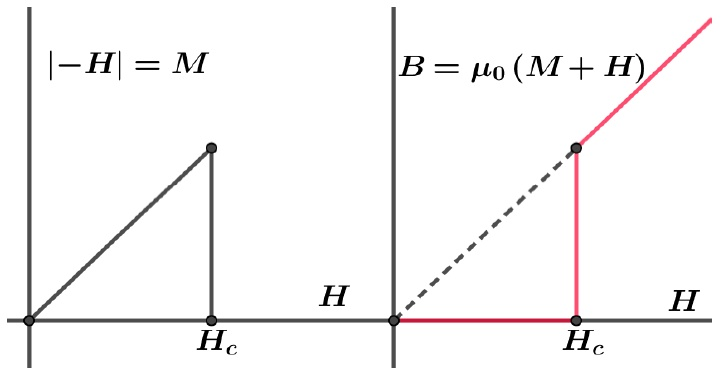
\includegraphics[width=0.6\textwidth]{./Figures/fig418}
	\caption{Relación entre $M$ y $H$}
	\label{fig:418}
\end{figure}

La primera limitación de los superconductores tipo I fue no solo debida a las bajas temperaturas, sino también al restringido rango en la densidad de corriente y el campo magnético, que era especialmente limitado en los primeros superconductores. Ejemplos son $Al$, $Ag$, $Hg$

Cómo fue visto existe una relación entre el campo magnético crítico y la temperatura crítica a la que Podemos agregar la densidad crítica de corriente. Las tres variables forman la superficie crítica, observamos en la gráfica. Estando la densidad crítica de corriente limitada a una capa superficial aproximadamente una décima de micrón. Siendo el campo máximo el que pueden operar aproximadamente 0,1 T . Hasta el momento estás restricciones limitan las posibles aplicaciones tecnológicas de los superconductores tipo I. Ver figura \ref{fig:419}

\begin{figure}[H]
    \centering
    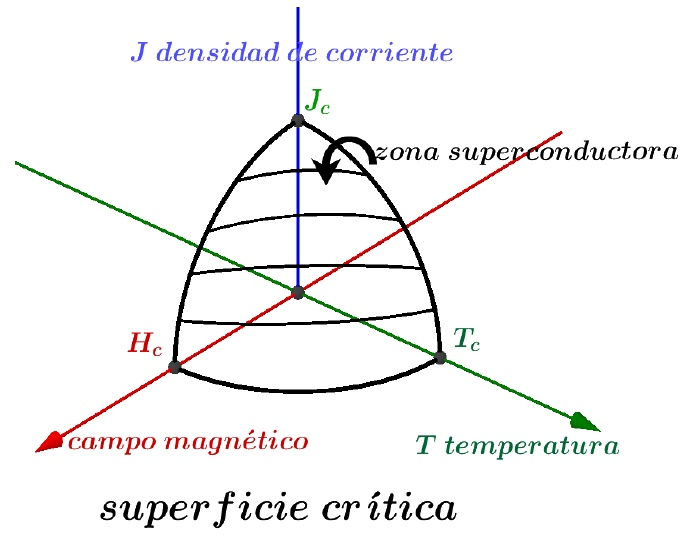
\includegraphics[width=0.6\textwidth]{./Figures/fig419}
	\caption{Relación entre $J$, $M$ y $H$}
	\label{fig:419}
\end{figure}


Existen también superconductores duros o tipo II, Se caracterizan por valores muy altos de los campos críticos y por una temperatura crítica mayor. Veamos alguna aclaración sobre energía superficial; la gran mayoría de los materiales tiene una energía superficial positiva, esto quiere decir, qué se debe invertir energía para formar una nueva superficie del material. Por el contrario si la energía superficial fuera negativa sería muy simple partir un material. Un estudio de Abrikosov (1957) sugirió que podría existir un tipo de superconductor con energía superficial negativa lo cual indicaría bajo ciertas condiciones espontáneamente se formarían superficies que separarían la parte normal de la superconductora en el material. De esta manera se la aparición del Estado mixto en un superconductor tipo II. Luego, el material superconductor se subdivide en una sucesión de regiones normales y superconductores cuyas fronteras son paralelas al campo magnético aplicado.

\subsection{Superconductores duros (tipo II)}

La diferencia fundamental entre ambos superconductores es que en el tipo II es posible la aparición de dos zonas. Dicho de otro modo; un superconductor tipo II es una mezcla de zonas (mixta) de conducción normal y superconductores. La intensidad del campo externo en el cual se conserva el estado mixto se denomina $H_{c2}$. Sí $H_{c1} < H < H_{c2}$ el flujo magnético penetra en el interior para formar regiones de flujo individual llamados vórtices. En la zona entre $H_{c2}$ y $H_{c1}$ el superconductor puede conducir corriente eléctrica dentro del material, de esta forma esta región del campo magnético puede ser usada para superconductores de alto campo y alta corriente. En este estado mixto de los superconductores tipo II no tiene lugar el efecto Meissner.

\begin{figure}[H]
    \centering
    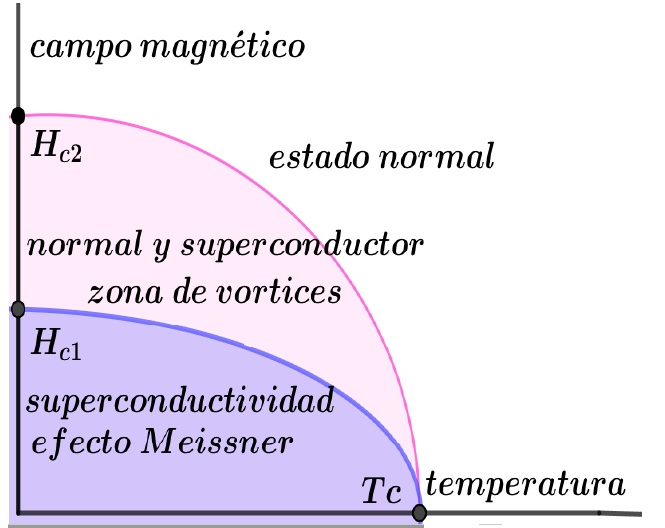
\includegraphics[width=0.5\textwidth]{./Figures/fig420}
	\caption{Superconductores tipo II}
	\label{fig:420}
\end{figure}

El superconductor tipo II, en el estado mixto; está atravesado por tubos de material en estado normal que son paralelos al campo magnético aplicado. Los tubos se distribuyen regularmente la estructura, dando a las propiedades del superconductor una regularidad equivalente. En cada tubo en estado normal hay una corriente que circula alrededor del tubo. La intensidad de vórtice aumenta al aumentar la intensidad de campo.


\begin{figure}[H]
  \begin{minipage}[b]{0.47\textwidth}
  Estos materiales son diamagnéticos, luego, al campo magnético aplicado se le opone otro campo magnético generado por una corriente superficial que circula en el perímetro de la muestra. En cada tubo dentro del material hay un flujo magnético que es generado por el vórtice de corriente que circula alrededor de cada tubo, el sentido es opuesto al de la corriente perimetral. En estos superconductores el campo magnético penetra solo en los tubos. Estas afirmaciones se observan en el esquema, en él, por simplicidad se dibujaron dos tubos. Observemos que los vórtices pueden ser interpretados como electroimanes con polaridad igual, lo cual indicaría que deberían repelerse entre ellos, este hecho determina la cantidad de vórtices existente en el material.
  \vspace{0.0cm}
  \end{minipage}
  \hfill
  \begin{minipage}[b]{0.47\textwidth}
     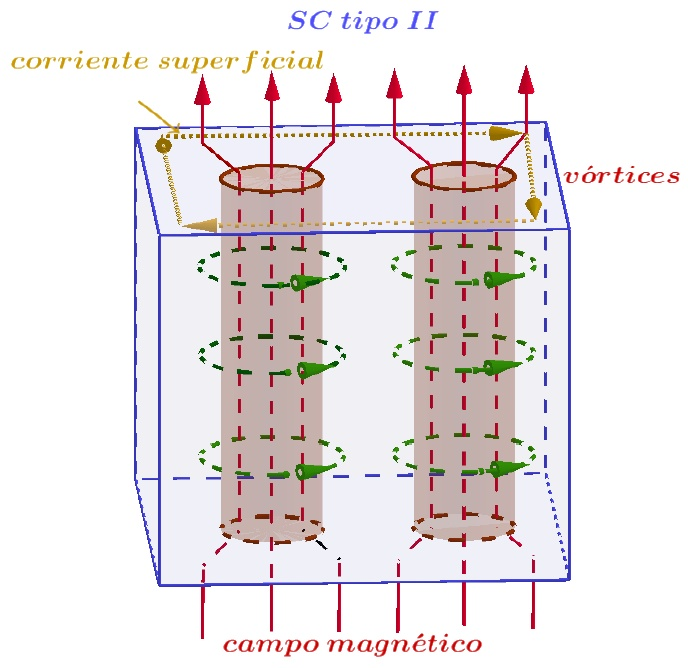
\includegraphics[width=1.10\textwidth]{./Figures/fig421}
     \caption{Vórtices en superconductores tipo II}
	\label{fig:421}
  \end{minipage}
\end{figure}

Estos superconductores también presentan ciclo de histéresis, no pareciéndose en nada ca los tradicionales. Los ciclos de histéresis se exteriorizan, cuando el material presenta defectos de distintos tipos: puntuales, lineales y volumétricos que impiden el movimiento de los vórtices, anclándolos. La visualización, por microscopia, de los vórtices muestra que no se ubican en el superconductor al azar, por el contrario, si el metal no tiene defectos los vórtices forman una estructura perfecta de simetría triangular. Si el sólido tiene defectos la red de los vórtices se verá distorsionada. Al aumentar el campo magnético crece el número de tubos de flujo, sobre los tubos actúa fuerzas de Lorentz que los hace migrar. Cada tubo se mueve con su flujo, esto implica una disipación de energía y por ende una resistencia eléctrica. La forma de evitar este movimiento es introduciendo defectos en el metal que anclan los vórtices, impidiendo su movimiento.

\subsection{Vórtices}

Aclaremos un poco más el comportamiento de los vórtices. Vórtice es sinónimo de Torbellino, vorágine da idea de un movimiento circular rápido. En la naturaleza se observan en distintas áreas y dimensiones, nuestro interés es en los vórtices microscópicos y que se producen a baja temperatura, no teniendo en cuenta los que son generados en fluidos cuánticos o superfluidos, caso del helio líquido. Nos ceñimos a aquellos que dan en la superconductividad.

vimos anteriormente que en el estado mixto o de vórtices existen zonas no superconductoras donde penetra el campo y se encuentran delimitadas por vórtices generados por la circulación de electrones superconductores que encierran al campo magnético. En el centro del vórtice los electrones se encuentran en el estado normal. Hay dos longitudes que caracterizan el vórtice y que dependen del material superconductor: $\varsigma$ la longitud coherencia que define la longitud de la zona central del vórtice y la longitud de penetración $\lambda$ (la calcularemos más adelante) que nos indica la penetración del campo fuera del tubo, (el campo y el flujo se encuentran en la zona normal, dentro del tubo) pasando este valor de $\lambda$ el campo es pequeño.

\begin{figure}[H]
  \begin{minipage}[b]{0.37\textwidth}
  En la figura \ref{fig:422} se representa la estructura de un tubo de flujo y el vórtice superconductor. Vemos también la curva de densidad de electrones superconductores en función de la distancia al centro del tubo, cero en el núcleo,(solo electrones normales en el núcleo), En azul el campo magnético con su longitud de penetración.
  \vspace{1cm}
  \end{minipage}
  \hfill
  \begin{minipage}[b]{0.57\textwidth}
     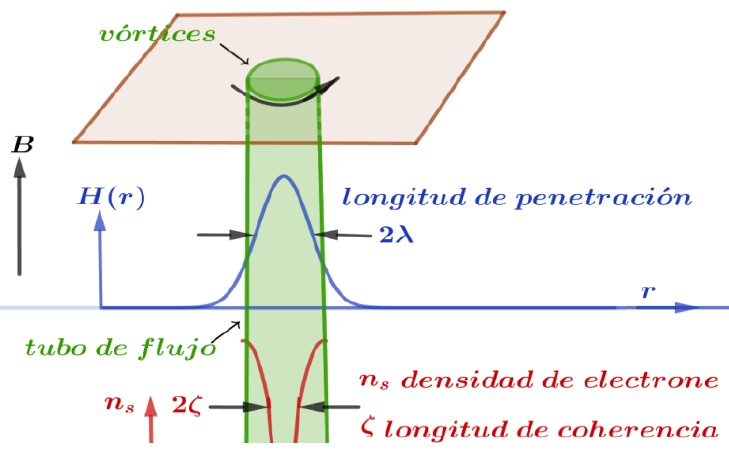
\includegraphics[width=1.0\textwidth]{./Figures/fig422}
     \caption{Vórtices en superconductores tipo II}
	\label{fig:422}
  \end{minipage}
\end{figure}



\begin{figure}[H]
  \begin{minipage}[b]{0.47\textwidth}
  En la figura \ref{fig:423} se observa la magnetización en función del campo, para los dos tipos de semiconductores, también vemos los vórtices, (en verde), indicando el aumento de estos hasta el final, cuando el material está en estado normal (totalmente verde indicando la penetración del campo).
  \vspace{2cm}
  \end{minipage}
  \hfill
  \begin{minipage}[b]{0.47\textwidth}
     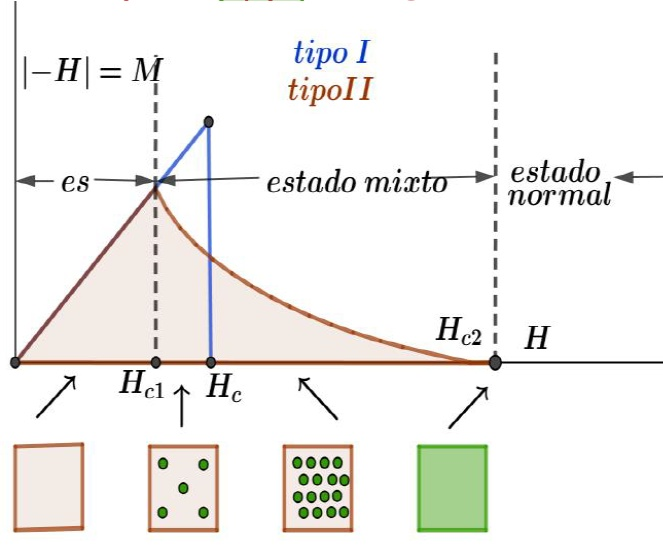
\includegraphics[width=1.10\textwidth]{./Figures/fig423}
     \caption{Megnetización en función del campo $H$ }
	\label{fig:423}
  \end{minipage}
\end{figure}

Este tipo de superconductor está hecho de aleaciones metálicas o de óxidos cerámicos complejos. Los más utilizados en imanes superconductores $Nb-Ti$ y $Nb3-Sn$, el campo crítico es $13 T$ y $27 T$ respectivamente y la densidad de corriente ${>10^{5}\frac{A}{cm^{2}}}$, comparada con ${\sim 10^{3}\frac{A}{cm^{2}}}$ para el hilo de cobre común.

las temperaturas críticas para $NbTi$ y $Nb_{3}Sn$ es de $10^{o}K$ y $18^{o}K$ respectivamente. el helio líquido puede enfriar a $42^{o}K$ a presión atmosférica, y tan bajo como $1,8^{o}K$ a presión reducida.

\subsection{Termodinámica de la superconductividad}

El estudio de un sistema puede hacerse de dos maneras macroscópicamente y microscópicamente, en muchos casos se complementan ambas descripciones. La termodinámica de un sistema es una descripción macroscópica del mismo. Si el sistema realiza un trabajo distinto de $p\,dV$, (eléctrico o magnético) debemos modificar las fórmulas. Sea $x_{j}$ e $y_{j}$ pares de magnitudes extensivas e intensivas acopladas. Puede en otros casos usarse otras variables equivalentes.

\begin{figure}[H]
    \centering
    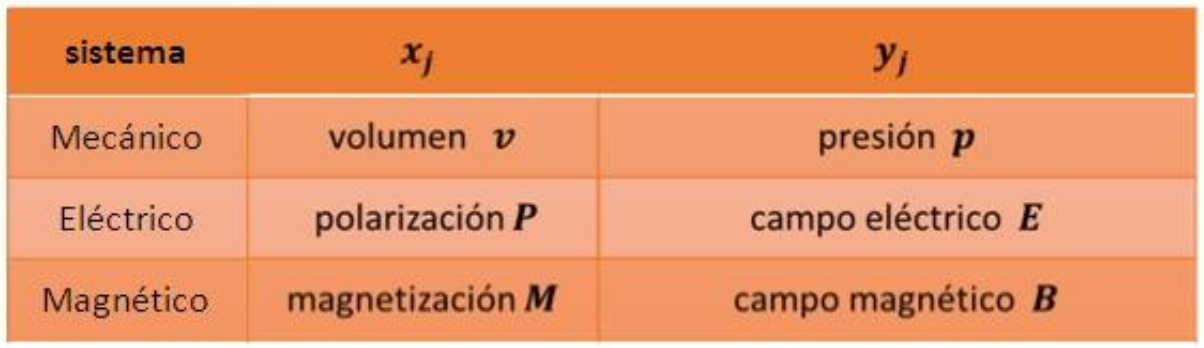
\includegraphics[width=0.9\textwidth]{./Figures/fig424}
	\label{fig:424}
\end{figure}

Luego la variación de energía interna la escribimos

\begin{equation}
dU=dQ+dW_{M}+dW_{e}+dW_{mag} = TdS-pdV+edP+BdM
\end{equation}

Los distintos potenciales termodinámicos serán:

\begin{equation}
F(T,x_{j}) , \quad G(T, y_{j})
\end{equation}

Energía libre de Helmholtz $dF=-Sdt+BdM$

Entalpía $d\Xi =  TdS - BdM$

Energía libre de Gibbs (magnética) $dG=-SdT-MdB$ o bien $dG=-SdT-BdH$

Luego resulta:

\begin{equation}
\begin{aligned}
  & \frac{\partial F}{\partial x_{j}} =y_{j}, \; \frac{\partial G}{\partial y_{j}} =x_{j} \quad \text{o sea}\\ 
  & \frac{\partial F}{\partial M} =B, \; \frac{\partial G}{\partial B} =M \quad  \text{Ecuación de Clausius}
\end{aligned}
\end{equation}

Estamos considerando sistemas en el que los efectos de las variaciones de presión y volumen son despreciables. Esto no siempre es así: un sistema puede cambiar su estructura cristalina con la temperatura y opresión. También supondremos que el trabajo químico es cero.

Siguiendo la deducción tradicional de la ecuación que gobierna los cambios de fase convencionales, tratamos de hallar la equivalente para la transformación superconductora normal.

En los cambios de fase se cumple la igualdad de la función de Gibbs en la curva Límite 

\begin{equation}
	G_{S}(H_{c}, T)=G_{n}(H_{c},t)
\end{equation}

Con la Gráfica de la figura \ref{fig:425}, se puede interpretar perfectamente el significado de lo que realizaremos.

\begin{figure}[H]
    \centering
    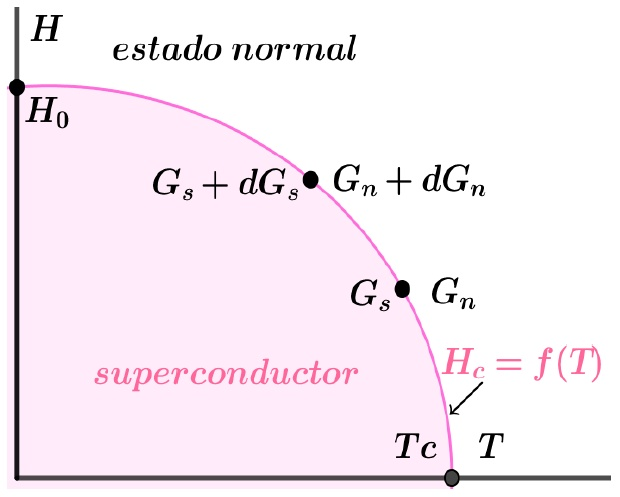
\includegraphics[width=0.5\textwidth]{./Figures/fig425}
	\caption{Separación de estados normal y superconductor}
	\label{fig:425}
\end{figure}

Partiendo de un estado donde coexisten las dos fases $G_{s}=G_{n}$ si el sistema evoluciona a lo largo de la curva $H_{c}=f(T)$ diferencialmente se cumple de nuevo la igualdad de las energías de Gibbs:

\begin{equation*}
	G_{S}(H_{c}, T) + dG_{S}(H_{c}, T) = G_{n}(H_{c},t)+ dG_{n}(H_{c},t)
\end{equation*}

Luego:

\begin{equation}
	dG_{S}(H_{c}, T) = dG_{n}(H_{c},t)
\end{equation}

por lo tanto tendremos:

\begin{equation}
\begin{aligned}
	dG_{s}(H_{c}, T) & = -S_{s}dT-B_{s}dH_{c} \\
	dG_{n}(H_{c}, T) & = -S_{n}dT-B_{n}dH_{c} \\
	-S_{s}dT-B_{s}dH_{c}  & = -S_{n}dT-B_{n}dH_{c} \\
	(B_{n}-B_{s})0dH_{c} & = (S_{s}-S_{n})dT \\
	\frac{dH_{c}}{dT} & = \frac{(S_{s}-S_{n})}{(B_{n}-B_{s})}
\end{aligned}
\end{equation}

\quad 1. Suponiendo que la mayoría de los metales son paramagneticos $M_{n}$ es despreciable, entonces $B_{n}=\mu_{0}H_{c}(T)$

\quad 2. Cómo $B_{n}=\mu_{0}(H_{c}+M_{s})$, pero $B_{s}=0$ por lo tanto:

\begin{equation}
\begin{aligned}
	\frac{dH_{c}}{dT} = -\frac{(S_{n}-S_{s})}{(B_{n}-B_{s})} & =  -\frac{(S_{n}-S_{s})}{\mu_{0}H_{c}(T)} \\
	S_{n}-S_{s} & = \mu_{0}H_{c}(T)\frac{dH_{c}}{dT}
\end{aligned}
\end{equation}

Qué es la ecuación de \textbf{Clausius-Clapeyron} para un material superconductor, esta ecuación permite caracterizar un cambio de fase de primer orden. El tercer principio de la termodinámica nos pide que $S_{n}-S_{s}$ se anulen en el cero absoluto, luego la derivada $\frac{dH_{c}}{dT}$ debe ser Cero en $T=0^{o}K$ y $\frac{dH_{c}}{dT} \neq 0$ para $T=T_{c}$. Por otra parte, si $T=0^{o}K$, $H_{c}(T)=H_{0}$ como no podemos llegar a $T=0^{o}K$ para llegar a $H_{0}$ se debe extrapolar.

Teniendo en cuenta que $l=T(S_{n}-S_{s}$ donde $l$ es el calor latente de la transformación, este calor latente representa una discontinuidad en la entropía durante la transición (Cambio de fase de primer orden). Es también el calor necesario para realizar la transformación, aunque no nos movamos del punto.

\begin{equation}
	l = T(S_{n}-S_{s}) = \mu_{0}TH_{c}(T)\frac{dH_{c}}{dT}
\end{equation}

Como Generalmente pasa en las transformaciones de primer orden el calor latente depende de la temperatura.

A presión y temperatura constante la energía libre para el súper conductor en función del campo magnético la hallamos de:



\begin{equation*}
dG=-Sdt-BdH \quad \text{integrando desde} \; H=0
\end{equation*}

\begin{equation*}
G_{s}(H, T)-G_{s}(0, T) = -\int_{0}^{H} B_{s}dH
\end{equation*}

De igual manera para el medio normal:

\begin{equation*}
G_{n}(H, T)-G_{n}(0, T) = -\int_{0}^{H} B_{n}dH
\end{equation*}

Entonces $G_{s}(H, T)-G_{n}(H, T)$ sobre la curva $H_{c}(T)$ será:

\begin{equation}
\begin{aligned}
[G_{s}(H, T)-G_{s}(0, T)]-[G_{n}(H, T)-G_{n}(0, T)] & = -\int_{0}^{H} B_{s}dH+\int_{0}^{H} B_{n}dH \\ 
& = \int_{0}^{H} (B_{n}-B_{s})dH \\
G_{s}(0, T)-G_{n}(0, T) &= \int_{0}^{H} (B_{n}-B_{s})dH 
\end{aligned}
\end{equation}

Como $B_{n}=\mu_{0}H_{c}(T)$ suponemos que la mayoría de los metales son paramagneticos y $M_{n}$ es despreciable y $B_{s}=\mu_{0}(H+M_{s})$ pero $B_{s}=0$ en toda la muestra, luego:


\begin{equation}
G_{s}(0, T)-G_{n}(0, T) = \int_{0}^{H}M_{s}dH =- \frac{\mu_{0}}{2}H_{c}^{2}
\end{equation}

Que es el área bajo la curva $M,H$. Tan solo para comprender los realizado se puede observar la figura \ref{fig:426}.

\begin{figure}[H]
    \centering
    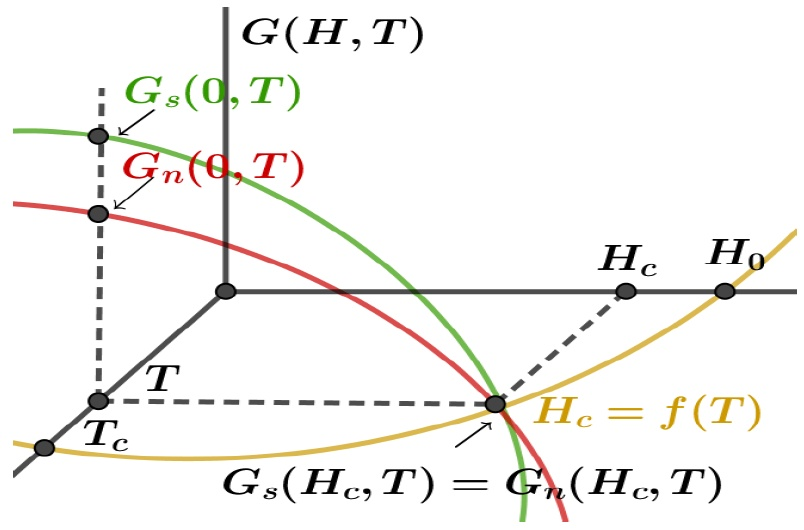
\includegraphics[width=0.5\textwidth]{./Figures/fig426}
	\caption{Equilibrio de estados en un superconductor}
	\label{fig:426}
\end{figure}


Como: $-S_{s}dT-B_{s}dH_{c}= -S_{n}dT-B_{n}dH_{c}$ en la curva $H_{c}=f(T)$ de coexistencia $B_{0}=0$ y $B_{n}=\mu_{0}H_{c}(T)$ despreciando $M_{n}$ entonces:

\begin{equation}
S_{n}-S_{s} = -\mu_{0} H_{c}(T) \frac{dH_{c}}{dT}
\end{equation}

Que es la ecuación de Clausius-Clapeyron para un material superconductor, la ecuación de Clausius-Clapeyron es una manera de caracterizar un cambio de fase de primer orden. Vemos que la derivada $\frac{dH_{c}}{dT}$ (ver figura \ref{fig:425} es siempre negativa entonces $S_{n}>S_{s}$ luego el estado superconductor es más ordenado que el normal.

Puesto que conocemos la función:

\begin{equation}
H_{c} = f(T_{c})=H_{0}\big( 1- \frac{T^{2}}{T_{c}^{2}}
\end{equation}

efectuando la derivada y multiplicando por $T$ hallamos el calor latente de la transformación $l=\Delta_{ns}$ 

\begin{equation*}
\frac{dH_{c}}{dT}=H_{0}\big( 1- \frac{T^{2}}{T_{c}^{2}} \big)
\end{equation*}

\begin{equation}
l=\Delta_{ns} = (S_{n}-S_{s})T=H_{0}\big( 1- \frac{T^{2}}{T_{c}^{2}}\big) H_{c}(T) = \frac{2\mu_{0}H_{0}^{2}T^{2}}{T_{c}^{2}}\big( 1- \frac{T^{2}}{T_{c}^{2}} \big)
\end{equation}

Como $l=\Delta_{ns}= (S_{n}-S_{s})T$ es el calor que se intercambia para pasar del Estado normal al superconductor $(n\rightarrow s)$ y como $S_{n}>S_{s}$, entonces se cede al entorno calor al pasar del normal al superconductor. Por el contrario se absorbe calor cuando $(n \leftarrow s)$

\subsubsection{Calor específico}

Como vimos que $S_{n}-S_{s}=-\mu_{0}H_{c}(T)\mfrac{dH_{c}}{dT}$ derivando ambos miembros respecto a $T$ y multiplicando por $T$

\begin{equation}
T\mfrac{dS_{n}}{dT}-T\mfrac{dS_{s}}{dT}=-\mu_{0}T\left[\left( \mfrac{dH_{c}(T)}{dT} \right)^{2} + H_{c}(T) \mfrac{d^{2}H_{c}(T)}{dT^{2}} \right] 
\end{equation}

Luego resulta:

\begin{equation}
C_{s}-C_{n}=\mu_{0}T\left[\left( \mfrac{dH_{c}(T)}{dT} \right)^{2} + H_{c}(T) \mfrac{d^{2}H_{c}(T)}{dT^{2}} \right] 
\end{equation}

Y si el campo aplicado es cero $H_{c}(T)=0$

\begin{equation}
C_{s}-C_{n}=-\mu_{0}T\left( \mfrac{dH_{c}(T)}{dT} \right)^{2}_{T=T_{c}}  
\end{equation}



Expresión que nos da la diferencia en el calor específico durante el Cambio de fase del estado superconductor al normal con campo 0, o sea, durante la transformación de segundo orden llamada \textbf{fórmula de Rutgers}.

También si recordamos que: $H_{c}=f(T_{c})=H_{0}\left(1-\frac{T^{2}}{T_{c}^{2}} \right)$ será:

\begin{equation}
C_{s}-C_{n}=\mu_{0}T\left( \mfrac{dH_{c}(T)}{dT} \right)^{2}_{T=T_{c}} =
 \mu_{0}T_{c}H_{0}^{2}\left( \frac{-T_{c}^{2}}{T_{c}^{2}} \right)^{2}= 4\mu_{0}T_{c}H_{0}^{2} 
\end{equation}

De donde podríamos hallar $H_{0}$ si conociéramos la diferencia de los calores específicos.

\subsubsection{Transformaciones de segundo orden}

vimos qué $S_{n}-S_{s}= -\mu_{0}H_{c}(T)\frac{dH_{c}}{dT}$ y como $S_{n}-S_{s}=\frac{l}{T}$ por lo tanto:

\begin{equation}
l= -\mu_{0}TH_{c}(T)\frac{dH_{c}(T)}{dT} 
\end{equation}

De esta última ecuación observamos claramente que sí $H_{c}(T)=0$ el calor latente también es cero y la entropía es continua $S_{n}=S_{s}$ lo cual indica que la transformación es de segundo orden.

En la figura \ref{fig:427} Se observa el cambio de la entropía en una transformación de segundo orden, siendo similar a una transformación tipo Lambda. La ecuación de Clausius-Clapeyron no es aplicable a las transformaciones de segundo orden.

\begin{figure}[H]
    \centering
    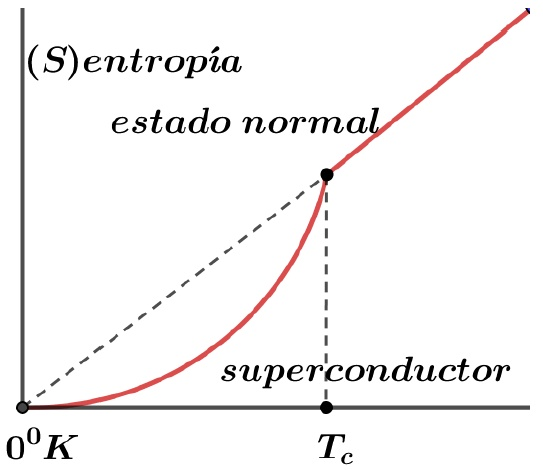
\includegraphics[width=0.5\textwidth]{./Figures/fig427}
	\caption{Transformación de 2° orden}
	\label{fig:427}
\end{figure}

\subsubsection{Transformaciones de fase}

\begin{figure}[H]
    \centering
    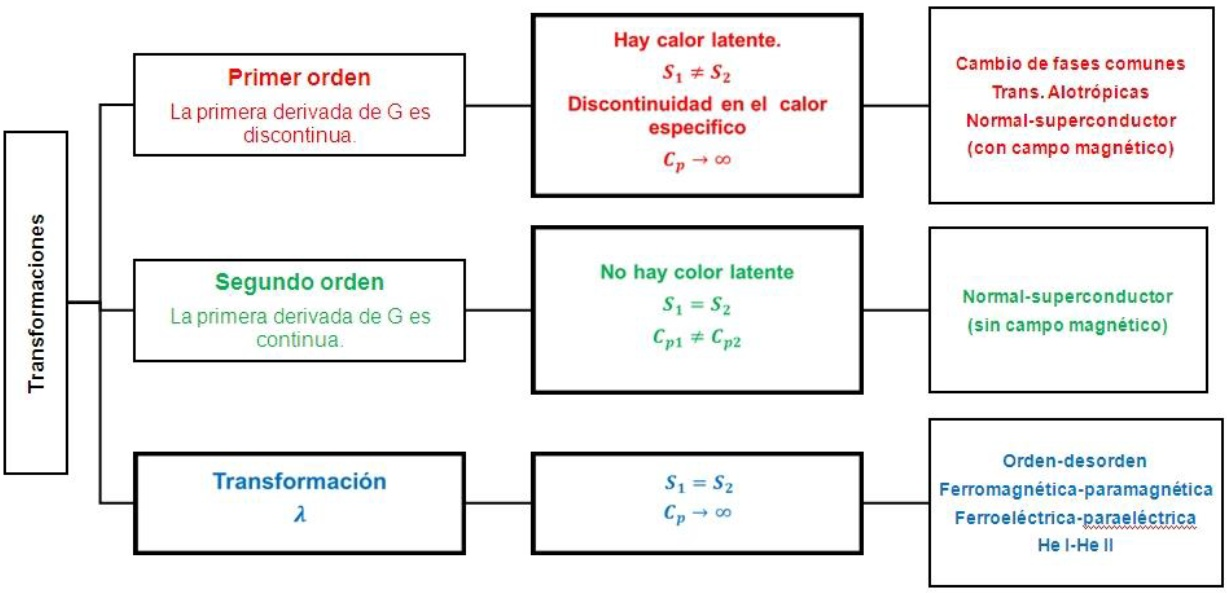
\includegraphics[width=1.0\textwidth]{./Figures/fig428}
	\caption{Transformación de fase}
	\label{fig:428}
\end{figure}

Estos gráficos, no pretenden ser más que esquemas donde se muestran el comportamiento teórico de la energía libre y el calor especifico en la zona de cambio de fase. Los cambios reales difieren en alguna medida, por razones que no son analizadas.

\begin{figure}[H]
  \begin{minipage}[b]{0.30\textwidth}
    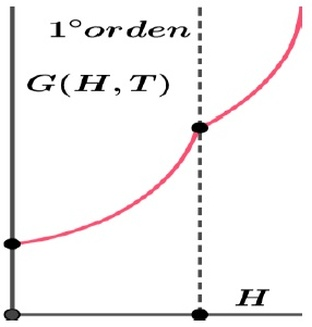
\includegraphics[width=1.0\textwidth]{./Figures/fig429}
	\label{fig:429}
  \end{minipage}
  \hfill
  \begin{minipage}[b]{0.30\textwidth}
    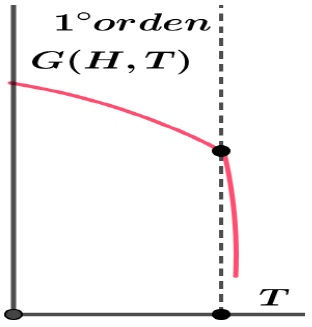
\includegraphics[width=1.0\textwidth]{./Figures/fig430}
	\label{fig:430}
  \end{minipage}
  \hfill  
  \begin{minipage}[b]{0.30\textwidth}
    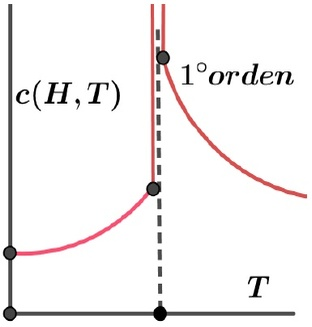
\includegraphics[width=1.0\textwidth]{./Figures/fig431}
	\label{fig:431}
  \end{minipage}  
\end{figure}


\begin{figure}[H]
  \begin{minipage}[b]{0.47\textwidth}
    \centering    
    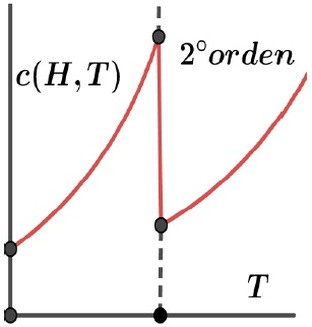
\includegraphics[width=0.6\textwidth]{./Figures/fig432}
	\label{fig:429}
  \end{minipage}
  \hfill
  \begin{minipage}[b]{0.47\textwidth}
	\centering
    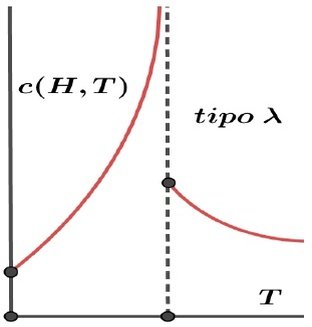
\includegraphics[width=0.6\textwidth]{./Figures/fig433}
	\label{fig:430}
  \end{minipage}
\end{figure}


\subsection{Frecuencia crítica}

Vimos en más de una oportunidad que a la temperatura crítica, sin campo magnético, hay una transformación de 2° orden y el calor específico presenta un pico, este comportamiento y estudios del aporte electrónico a la capacidad calórica, lleva a pensar en la existencia de una banda prohibida de energía. En la figura se observa el esquema de bandas de energía para un metal común y para un superconductor. Los valores típicos de $E_{g}\approx 10^{-4}eV$ (bandas exageradas en la figura \ref{fig:434}). Se vio anteriormente que existe la temperatura crítica, el campo crítico y la corriente crítica. Estamos ahora en condiciones de introducir la frecuencia crítica $F_{c}$. Si un superconductor se encuentra en un campo electromagnético variable mantiene sus propiedades Sólo hasta las frecuencias inferiores a $10^{11}Hz$, llamada frecuencia crítica. Luego de la cual su resistencia aumenta, volviéndose normal. Este comportamiento es también explicable por la teoría los dos fluidos, sabemos que los Súper electrones tienen menor energía que los electrones normales. luego, si la frecuencia de los fotones de la onda electromagnética tienen la energía suficiente para excitar a los Súper electrones y pasarlos a electrones normales, el material dejaría de ser superconductor. De otro modo; los fotones con energía $>E_{g}$ provocarían la transición de electrones a niveles energéticos desocupados por encima de la banda prohibida.

\begin{figure}[H]
    \centering
    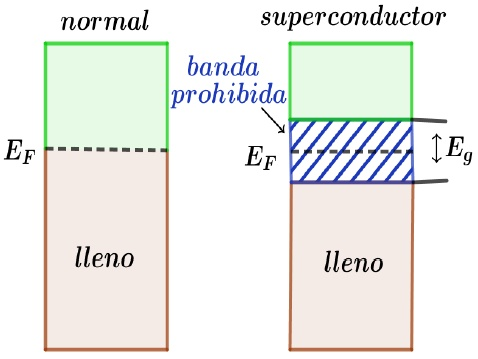
\includegraphics[width=0.5\textwidth]{./Figures/fig434}
	\caption{Conductor normal y superconductor}
	\label{fig:434}
\end{figure}

Este comportamiento no crea inconvenientes en las aplicaciones comunes de los superconductores, ya que las frecuencias de estos casos son muchos menores.

\subsection{Teoría de los dos fluidos}

En 1908 Heike K. Onnes Puedo licuar helio, aunque no consiguió solidificarlo, hecho que sucedió en 1926, en 1911 descubre la superconductividad. Si los avances experimentales para obtener bajas temperaturas No se podría haber descubierto la superconductividad. La primera descripción teórica (clásica) sobre el tema fue propuesta en 1935 por los hermanos London. Interesante destacar la esencia de estos hechos: una realización experimental permite el descubrimiento de un nuevo fenómeno, el cual conlleva a una propuesta teórica. Sin embargo, No termina allí la secuencia. El helio líquido, logrado primitivamente por Onnes, demostró tener propiedades especiales, tal es así, qué en 1937 Piotr Kapitsa (se hizo famoso en 1946 al enfrentarse a Stalin y no querer trabajar en el desarrollo de armas nucleares), descubre la superfluidez del helio. Dicho de otro modo, ausencia de viscosidad, lo cual, vence cualquier intento de ser contenido en un recipiente, El helio escapa del vaso que intenta contenerlo.
Anteriormente, en el tema de la magnetorresistencia, concretamente en conducción eléctrica, sin mencionarlo específicamente hablamos de la \textbf{ley de Drude}. el modelo supone que el campo eléctrico ejerce una fuerza existiendo otra fuerza opuesta similar a una fricción proporcional a la velocidad, dando

\begin{equation}
	m\mfrac{d\overrightarrow{v}}{dt}=e\overrightarrow{E}-\gamma \overrightarrow{v}
\end{equation}

La solución estacionaria es $\overrightarrow{v}=\left(\mfrac{e}{\gamma} \right) \overrightarrow{E}$ sí $\gamma=\left(\mfrac{m}{\tau} \right)$ siendo $\tau$ el tiempo de vuelo medio. Suponiendo que para $T<T_{c}$ tenemos dos tipos de electrones, (dos fluidos): los superconductores y los comunes, cuyas densidades son $n_{s}$ y $n_{n}$, siendo la densidad total $n=n_{s}+n_{n}$.

Para $T\rightarrow 0$, $n_{s}\rightarrow n$ mientras que para $T\rightarrow T_{c}$, $n_{s}\rightarrow 0$. Los electrones normales conducen con resistencia finita mientras que los electrones superconductores conducen sin disipación. 

La ecuación de P. Dude $m\frac{dv}{dt} = eE-\frac{mv}{t}$ queda trabajando sólo con los electrones superfluidos:

\begin{equation}
	\mfrac{d\overrightarrow{v}}{dt}=\frac{e}{m}\overrightarrow{E} \quad \text{¿Por qué de esta manera?}
\end{equation}

Si reemplazamos la ley de Ohm por una súper corriente $J_{s}=n_{s}ev_{s}$ nos queda:

\begin{equation}
	\mfrac{\partial \overrightarrow{J_{s}}}{\partial t}=\frac{n_{s}e^{2}}{m}\overrightarrow{E} \quad \text{o bien} \quad \overrightarrow{E}= \frac{m}{n_{s}e^{2}} \mfrac{\partial \overrightarrow{J_{s}}}{\partial t} \text{llamada 1° ecuación de London}
\end{equation}

Atención reemplacé la derivada total por otra parcial ¿que se supuso? ver ejercicio N°. . .

Tomando rotor en ambos lados de la ecuación

\begin{equation}
	\nabla \times \overrightarrow{E} = \frac{m}{n_{s}e^{2}} \nabla \times \mfrac{\partial \overrightarrow{J_{s}}}{\partial t} = -\mfrac{\partial B}{\partial t}
\end{equation}

De acuerdo con la ecuación de Maxwell, se puede escribir:


\begin{equation}
	\frac{\partial}{\partial t}\left( \frac{m}{n_{s}e^{2}}\nabla \times \overrightarrow{J_{s}} + \overrightarrow{B}  \right) = 0 \; text{luego} \frac{m}{n_{s}e^{2}}\nabla \times \overrightarrow{J_{s}} + \overrightarrow{B} = Ctte \quad \text{llamada 2° ecuación de London}
\end{equation}

Como el campo magnético y la corriente son nulos en el interior del superconductor la constante vale cero, por tanto:

\begin{equation}
\label{eq:40}
\frac{m}{n_{s}e^{2}}\nabla \times \overrightarrow{J_{s}} + \overrightarrow{B} = 0
\end{equation}

\subsubsection{Ecuación de London}

Tratemos de llegar a una ecuación diferencial en $\overrightarrow{B}$, para ello recurrimos nuevamente a Maxwell, en este caso a la siguiente expresión:

\begin{equation*}
	\nabla \times \overrightarrow{B} = \mu_{0}\overrightarrow{J_{s}}
\end{equation*}

y tomando rotor en ambos miembros:

\begin{equation*}
	\nabla \times \nabla \times \overrightarrow{B} = \mu_{0}\nabla \times \overrightarrow{J_{s}} \;\text{como:}\;
	\nabla \times (\nabla \times \overrightarrow{B})= \nabla (\nabla \cdot \overrightarrow{B}) - \nabla^{2} \overrightarrow{B}  \;\text{y como}\; \nabla \cdot \overrightarrow{B} =0 \;\text{queda}\;
\end{equation*}

\begin{equation*}
	\nabla \times (\nabla \times \overrightarrow{B})= - \nabla^{2} \overrightarrow{B} = \mu_{0} \nabla \times \overrightarrow{J_{s}}  \;\text{luego:}
\end{equation*}

\begin{equation*}
	\nabla \times \overrightarrow{J_{s}}=\frac{ \nabla^{2} \overrightarrow{B}}{\mu_{0}}
\end{equation*}

Reemplazando en la ecuación \ref{eq:40} nos queda la 

\begin{equation}
\label{eq:41}
	\frac{m}{\mu_{0}n_{s}e^{2}}\nabla^{2} \overrightarrow{B} + \overrightarrow{B} = 0 \; \text{Ecuación de Banner}
\end{equation}

Esta ecuación explica las condiciones del campo para que exista el efecto Meissner:


\begin{itemize}
	\item Campo magnético nulo en superconductor.
	
	\item La corriente eléctrica limitada a una capa superficial de espesor $\lambda$, en el resto del conductor es cero. Como demostraremos seguidamente

\end{itemize}

\subsection{Profundidad de penetración del campo y corriente}

Teniendo en cuenta la ecuación de Banner \ref{eq:41} y llamando $\lambda=\sqrt{\frac{m}{\mu_{0}n_{s}e^{2}}}$

Observamos que al resolver la ecuación diferencial el campo penetra una distancia $\lambda$ decayendo exponencialmente. El parámetro $\lambda$ es llamado profundidad de penetración

De la misma ecuación \ref{eq:41} también obtenemos que la corriente de apantallamiento se encuentra localizada a una distancia $\approx \lambda$. Cuando aplicamos un campo a un superconductor la corriente que Cancela este campo penetra aproximadamente una distancia $\lambda$ en el conductor. Explica que el campo en el interior del metal debe ser nulo, ya que es una de las hipótesis del desarrollo anterior, y que existe una corriente limitada a un espesor de la superficie de superconductor, cuyo espesor es del orden de $10^{−7}m$ dependiendo de superconductor. Posteriormente se encuentra que estos resultados no son del todo correctos. Una de las hipótesis que no es correcta es la suposición de que los electrones individuales son los responsables de la conducción eléctrica, lo cual se vio que era erróneo varias décadas después. Sin embargo, a pesar de este rollo inicial, los resultados experimentales no se vieron muy afectados. Tratemos de aclarar esta situación.

Basándose en resultados experimentales, Cooper (1956) propone que los portadores de carga no son en realidad los electrones individuales, sino parejas de electrones, llamados pares de Cooper, Posteriormente la teoría llamada \textbf{BCS} lo Explica en detalle. Los pares de Cooper son cuasiparticulas formadas por dos electrones, por lo tanto la masa $m=2m_{e}$ la carga $q=2q_{e}$. Cuando un electrón se mueve en una estructura superconductora distorsiona ligeramente la red de iones positivos generando Un aumento local de densidad de carga positiva que atrae al segundo electrón. El estado superconductor los electrones se hallan ligados por intermedio de la red cristalina y ambas partículas funcionan como si sea trajeran pese a que tienen igual signo sus cargas. Por tanto, los iones del material se acoplan con el movimiento de los electrones que se mueven dentro de él. Luego el arreglo de átomos de superconductor comienza a oscilar de manera periódica y coordinada con el movimiento de los electrones. En este movimiento coordinado no hay pérdida de energía.

\begin{figure}[H]
    \centering
    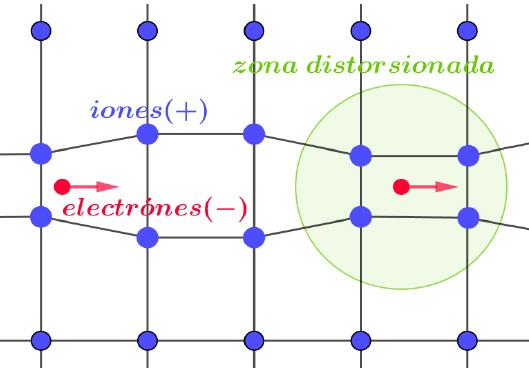
\includegraphics[width=0.5\textwidth]{./Figures/fig435}
	\caption{Pares de Cooper}
	\label{fig:435}
\end{figure}

La figura \ref{fig:435} es tan sólo un esquema que ejemplifique lo mencionado en el texto


\subsection{Cuantificación del flujo y fluxoides}

Las ecuaciones de London constituyen un modelo fenomenológico y clásico. Mentalmente explica los superconductores tipo I, pero nada dice sobre la penetración y cuantificación de flujo en los conductores tipo II, Este caso es un fenómeno cuántico. Existen diversas maneras de acceder a la idea de cuantificación del flujo, sin hacer una demostración cuántica rigurosa. En 1950 Vitali Ginzburg y Lav landau proponen una teoría macroscópica aplicable a los superconductores de alta temperatura. Dicho de otro modo, con regiones superconductoras y normales tipo II, siendo está, una generalización de la teoría de London.

En la teoría se propone la función de onda macroscópica $\Psi$ o seudofunción de onda, ya que no es la solución de la ecuación de Schródinger, sin embargo, respeta varias de las propiedades de la función de onda. La podemos pensar como una función de onda macroscópica.

Se interpreta a $\vert \Psi  \vert^{2}=n_{s}$ como la densidad de carga de los portadores superconductores, o sea densidad de pares de Cooper. En la mecánica clásica una onda se corresponde con algo que oscila así nos indica lugar del oscilación nos encontramos. En una onda cuántica la interpretación de la fase es más compleja, pues no hay nada que hacer. Cada par de Cooper puede ser tratado como una partícula con masa y carga igual al doble del electrón. La función de onda del electrón en un sólido suele ser muy corta debido a la dispersión que sufren los electrones al moverse el conductor, cambiando las fases de la función de onda De manera azarosa. Luego si conocemos la función de onda en un punto no significa que se la pueda conocer en otra posición.

En los superconductores los portadores son los pares de Cooper y no sufren dispersión, esto significa que hay coherencia de fase a larga distancia, del orden de $10^{-4}cm$. Cuando un metal se convierte en súper conductor la onda que describe las propiedades de los portadores cubre todo el objeto y una sola onda corresponde a todos los portadores del sistema esta onda de una fase qué llamamos $\varphi$.

La función de onda puede escribirse como:

\begin{equation}
	\Psi=\Psi_{0}e^{\frac{i(\vec{P},\vec{r}}{h}}
\end{equation}

La coherencia de largo alcance permite calcular la fase y la amplitud de la función de onda en cualquier punto a partir de un valor en un punto de referencia. La coherencia cuántica son estados que mantienen la fase una cierta distancia y posibilita el fenómeno de interferencia. la variación de fase a lo largo de una cerrada del tipo $C$ debe ser múltiplo de $2\pi$ para que la función de onda sea unívoca. La función de onda la podemos escribir como una onda unidimensional

\begin{equation}
	\Psi =  Real \left[ \Psi_{0}e^{\frac{i(\vec{k}\cdot \vec{r}-\omega t}{h}}\right] 
\end{equation}

%$\mathbb{R} $

La frecuencia está vinculada con la energía del par y la longitud de onda $lambda$ con el impulso $\lambda= \frac{h}{p}$. La diferencia de fase entre dos puntos a y b de un superconductor se puede calcular de la siguiente manera $k(a-b)$, qué integrando para una curva cualquiera nos da la circulación.

\begin{equation}
	\Delta\varphi_{a,b}=\varphi_{a}-\varphi_{b}=\int_{a}^{b}\overrightarrow{k}\cdot \overrightarrow{dl} 
\end{equation}

en un círculo cerrado para que haya coherencia de fase debe ser igual a $2\pi n$. Sabemos que la cantidad de movimiento para un electrón libre es $p=mv=\hbar k$ por lo tanto para un par de Cooper será $\hbar k = 2mv$ vimos que:

\begin{equation}
	J_{s}=n_{s}ev_{s} \Rightarrow k= \frac{2mJ_{s}}{\hbar n_{s} e}
\end{equation}

y si es superconductor no es simplemente conexo, por ejemplo un anillo, debe existir coherencia de la función de onda y la fase debe tomar el mismo valor luego de un giro completo

\begin{equation}
	\oint k \cdot dl= \oint \frac{2mJ_{s}}{\hbar n_{s} e} \cdot dl = \frac{2m}{\hbar n_{s} e} \oint J_{s} \cdot dl = \frac{2m}{\hbar n_{s} e} \iint(\nabla \times J_{s}) \cdot ds
\end{equation}

donde hemos aplicamos el teorema de Stokes. Y si ahora tenemos en cuenta la segunda ley del London:

\begin{equation}
\begin{aligned}
\label{eq:flujoCuantizado}
	& \frac{m}{n_{s} e^{2}} \nabla \times J_{s} + B =  \frac{m}{\mu_{0} n_{s} e^{2}} \nabla^{2} B+B=0 \\
	& \frac{2m}{\hbar n_{s} e} \iint \left(\frac{n_{s}e^{2}}{m}B \right) \cdot ds = \frac{2e}{\hbar} \iint B \cdot ds = 2\pi \\
	& \frac{2e}{\hbar} \Phi_{0} = 2\pi \Rightarrow \Phi_{0} = \frac{2\pi\hbar}{2e} = \frac{h}{2e} = 2,0678.10^{-15} \left[ \frac{Tesla}{m^{2}} \right] 
\end{aligned}
\end{equation}


\begin{figure}[H]
    \centering
    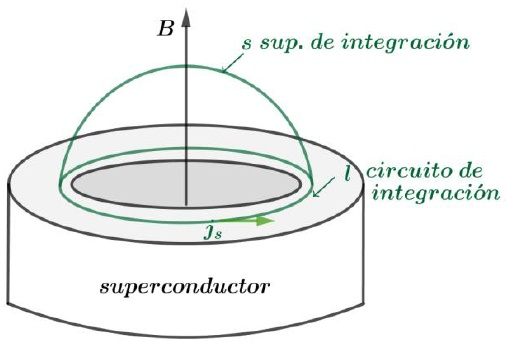
\includegraphics[width=0.5\textwidth]{./Figures/fig436}
	\caption{Integración del flujo $\Phi_{0}$}
	\label{fig:436}
\end{figure}

La integral de superficie es el flujo $\Phi_{0}$ del campo $B$ producida por la súper corriente. Partimos de la unicidad de la función de onda y de la periodicidad de la fase y llegamos a la cuantificación del flujo.

A veces el flujo producido por la súper corriente es llamado flujo interno.

El flujo magnético que pasa a través del superconductor está cuantificado y siempre es un múltiplo entero de , $\Phi_{0}=\frac{h}{2e}$ llamado fluxsoide. Al decir que está cuantificado indicamos que sólo puede valer un número entero de veces el fluxoide.

Discuta el caso siguiente: enfriamos un anillo superconductor en un pequeño campo magnético que genera un flujo $\Phi_{0}$ luego sacamos el campo magnético, ¿que pasa?


\subsection{Efecto Josephson}

En 1962 J. D. Josephson predijo la aparición de una corriente eléctrica por efecto túnel entre dos superconductores separados por una barrera aislante fina (juntura), un año después fueron construidas. Pensemos en dos electrodos metálicos de niobio aislados, por una barrera delgada de unos pocos nanómetros de óxido de aluminio. En la figura \ref{fig:437} se observan los dos tipos de juntura Josephson.

\begin{figure}[H]
    \centering
    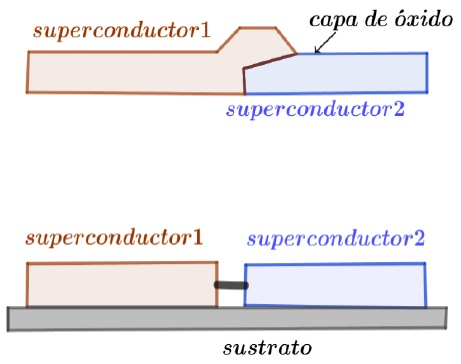
\includegraphics[width=0.5\textwidth]{./Figures/fig437}
	\caption{Efecto Josephson}
	\label{fig:437}
\end{figure}

Si la temperatura es $T>T_{c}$ (para el niobio $T_{c}=9,9^{o}K$) la juntura se comporta como una resistencia común que sigue la ley de Ohm. Por debajo de la temperatura crítica $T_{c}$, el niobio se vuelve superconductor, se generan pares de Cooper. Los pares de Cooper no existen en un aislante o en un metal no superconductor, cuando la capa que separa las dos superconductores es estrecha, los pares pueden atravesarla. Las expresiones que gobiernan este fenómeno son:

Entre ambos superconductores establece la siguiente corriente 

\begin{equation}
	I=I_{0}Sin(\Delta\varphi)
\end{equation}

donde $\Delta\varphi$ es la diferencia de fase entre las funciones de onda en los dos superconductores y es la máxima corriente que puede soportar el sistema. La corriente fluye de un bloque hacia el otro sin que sea preciso que exista diferencia de potencial mi campo magnético aplicado entre uno y otro. Este efecto es llamado \textbf{Efecto Josephson DC}

En la figura \ref{fig:438} se observa una juntura Josephson con las funciones de onda y las ecuaciones fundamentales. Si los dos superconductores están suficientemente próximos actuarán como si fueran un solo superconductor ( acoplamiento débil). Este tip o de acoplamiento se puede lograr por medio de contactos tipo punta, óxidos poco conductores y en algunos casos con límites de granos cristalograficos.

\begin{figure}[H]
    \centering
    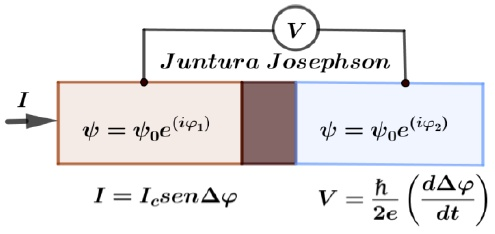
\includegraphics[width=0.5\textwidth]{./Figures/fig438}
	\caption{Juntura Josephson}
	\label{fig:438}
\end{figure}


Además se determinó que si se mantenía una diferencia de potencial $V$ en la juntura entonces $\Delta\varphi$ evoluciona según:

\begin{equation}
	\frac{d(\Delta\varphi)}{dt}= \frac{2eV}{\hbar}
\end{equation}

llamado \textbf{Efecto Josephson AC}. Vemos que:

\begin{equation}
	\frac{(d\Delta\varphi)}{dt} = \frac{2\pi}{\hbar}(V_{1}-V_{2})\rightarrow \text{integrando}\rightarrow \varphi=\frac{2\pi}{\hbar}(V_{1}-V_{2}) T + \varphi_{0}
\end{equation}

reemplazando en $I= I_{0}Sin(\Delta\varphi)$


\begin{equation}
	I=I_{0}Sin\left( \frac{2\pi}{\hbar}(V_{1}-V_{2}) T + \varphi_{0}\right) 
\end{equation}


luego la aplicación de una diferencia de potencial produce una corriente superconductora de una frecuencia:
 
\begin{equation}
	\frac{2e}{\hbar}(V_{1}-V_{2})
\end{equation}

Y por tanto es un convertidor voltaje-frecuencia.

En la figura \ref{eq:439} vemos la característica corriente-tensión de una juntura Josephson a diferentes temperaturas:

\begin{figure}[H]
    \centering
    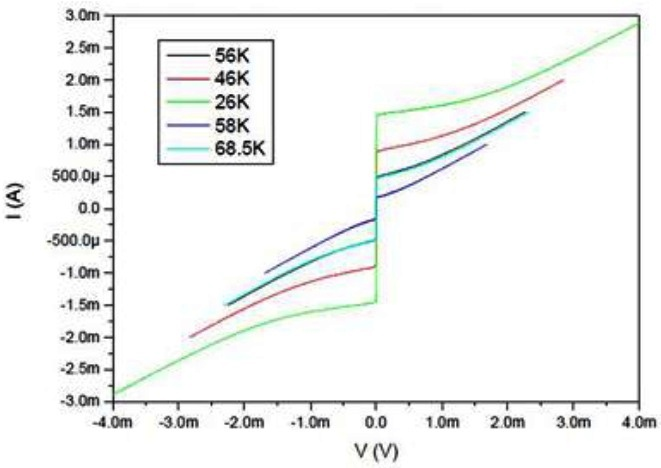
\includegraphics[width=0.7\textwidth]{./Figures/fig439}
	\caption{Juntura Josephson}
	\label{fig:439}
\end{figure}


\subsection{Interferencia cuántica - Squid}

Una de las aplicaciones de las junturas Josephson y quizás la más conocida, es el magnetómetro Squid. Su sigla en inglés que significa \textit{Superconducting Quantum Interference Devices}. Este instrumento es un medidor de campo magnético muy sensible basado en una o dos uniones Josephson dependiendo del tipo.

Comentaremos sólo el de 2 uniones, este sistema está constituido por dos uniones superconductoras idénticas en paralelo. En ausencia de campo magnético externo, se aplica una corriente $I$, corriente de polarización. La corriente se divide en dos, $\frac{1}{2}$ en cada rama.

En las uniones tipo Johnson se produce un Cambio de fase $\Delta\varphi$. No hay diferencia de potencial a través de ellas, siempre que $\frac{I}{2}$ no supere la corriente crítica. Se sabe que la aplicación de un campo magnético en un superconductor produce un Cambio de fase en la corriente $I_{c}$. Al introducir un campo magnético se genera una súper corriente $I_{s}$ que crea un campo que se opone al flujo externo aplicado. Dado que el Cambio de fase alrededor del anillo debe ser un múltiplo de $2\pi$ para mantener valor único de la función de onda la cantidad de flujo dentro del anillo sólo puede tener valores discretos. La corriente será:

\begin{equation*}
	\frac{I}{2}+ I_{s} = I_{c} Sin(\Delta\varphi+\delta)
\end{equation*}

en una rama, mientras que en la otra será:

\begin{equation*}
	\frac{I}{2}+ I_{s} = I_{c} Sin(\Delta\varphi-\delta)
\end{equation*}

Sumando obtenemos $I = 2I_{c}Cos(\delta)Sin(\Delta\varphi)$ dónde $\Delta\varphi$ es el cambio de fase debido a la súpercorriente. Ver figura \ref{fig:442b}

\begin{figure}[H]
    \centering
    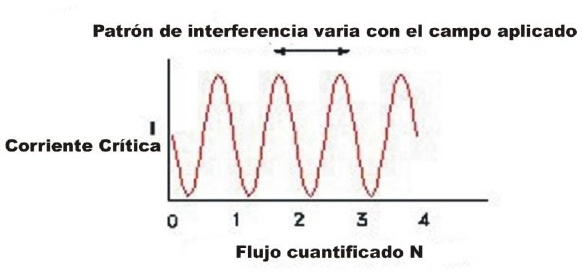
\includegraphics[width=0.8\textwidth]{./Figures/fig442b}
	\caption{Squid interferencia}
	\label{fig:442b}
\end{figure}


Analicemos un poco más el fenómeno. En la figura \ref{fig:440} observamos un esquema que representa al Squid sin campo externo y con el.

\begin{figure}[H]
    \centering
    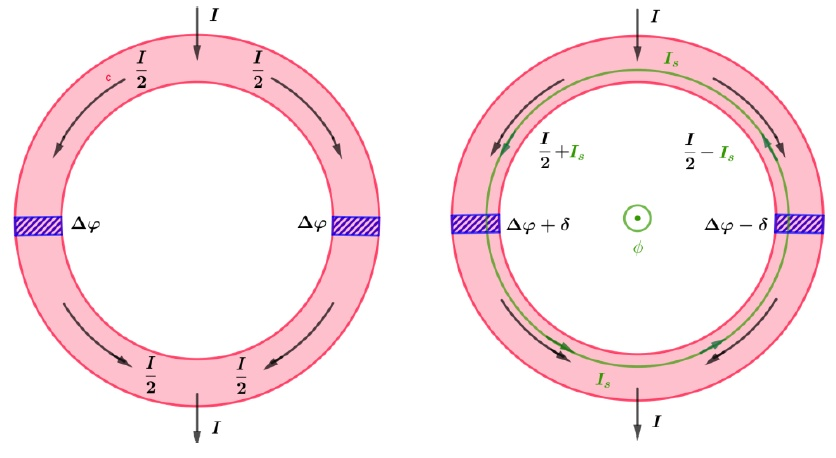
\includegraphics[width=0.9\textwidth]{./Figures/fig440}
	\caption{Squid con y sin campo externo}
	\label{fig:440}
\end{figure}

\subsubsection{Squid en un campo externo}

Tan pronto como la corriente en cualquiera de las ramas excede a la corriente crítica de la unión Josephson, aparece un voltaje a través de la unión tal como se ve en la figura \ref{fig:441}. Analicemos el caso en que un campo externo es aplicado al Squid. En presencia de un campo magnético el momento se modifica de la siguiente forma $P=mv+eA$ que para los pares de Cooper toma la forma siguiente $P=mv+eA= k\hbar$, siguiente Siendo $A$ el potencial vectorial magnético. 

\begin{figure}[H]
    \centering
    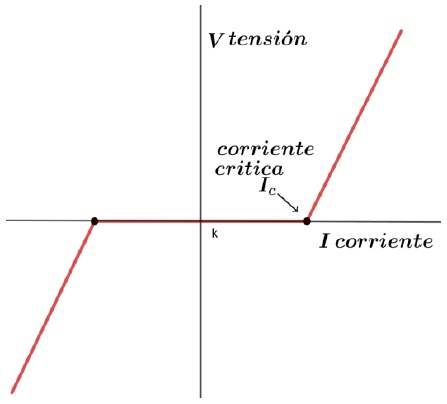
\includegraphics[width=0.5\textwidth]{./Figures/fig441}
	\caption{Squid con y sin campo externo}
	\label{fig:441}
\end{figure}


Haciendo un razonamiento similar al realizado cuando se vio la cuantificación del flujo (\ref{eq:flujoCuantizado}):

\begin{equation*}
	\oint k \cdot dl = \oint \frac{2mJ_{s}}{\hbar n_{s} e} \cdot  dl = \oint \frac{2e}{\hbar} A \cdot dl = 2\pi n
\end{equation*}

pos Stokes

\begin{equation*}
	\frac{2m}{\hbar n_{s} e} \iint \nabla \times J_{s} \cdot  ds  = \frac{2e}{\hbar} \iint \nabla \times A \cdot ds = 2\pi n
\end{equation*}

Aquí en necesario distinguir entre los dos campos magnéticos, el producido por $J_{s}$ y el colocado desde afuera proveniente de $A$.

Pero como:

\begin{equation*}
	\frac{2m}{\hbar n_{s} e} \nabla \times J_{s}   = -B_{int} \quad \text{y} \quad  \nabla \times A = B_{ext}
\end{equation*}

Entonces resulta:

\begin{equation*}
	\frac{-2e}{\hbar} \iint B_{int} \cdot  ds  + \frac{2e}{\hbar} \iint B_{ext} \cdot ds = 2\pi n
\end{equation*}

\begin{equation*}
	\frac{-2e}{\hbar}(\Phi_{ext}-\Phi_{int} ) = 2\pi n
\end{equation*}

\begin{figure}[H]
    \centering
    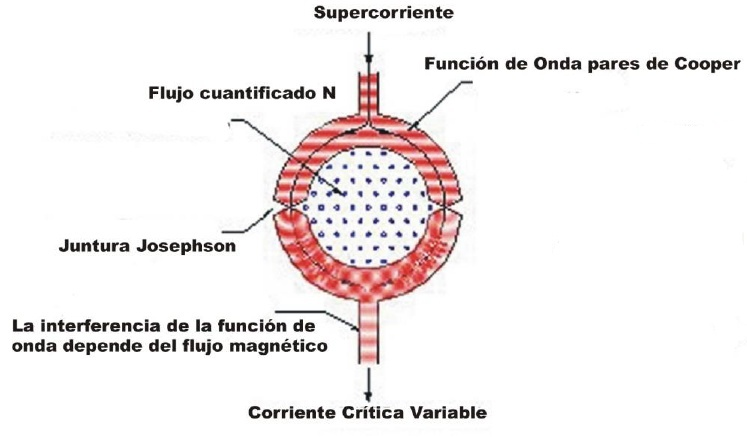
\includegraphics[width=0.9\textwidth]{./Figures/fig442a}
	\caption{Squid interferencia}
	\label{fig:442a}
\end{figure}

\subsubsection{Aplicaciones}

Los superconductores tienen numerosas aplicaciones. Actualmente, los imanes más potentes se fabrican con bobinas de cables superconductores, seguidamente mencionamos algunas de ellas.

\begin{itemize}
	\item Medicina: En los equipos de \textbf{RMN} (Resonancia Magnética Nuclear), es necesario orientar el momento magnético, (hidrogeno), en la dirección de un campo magnético. Esto se logra por medio de bobinas superconductoras. Este instrumento es de uso común en hospitales y en diagnóstico médico.
	
\begin{figure}[H]
    \centering
    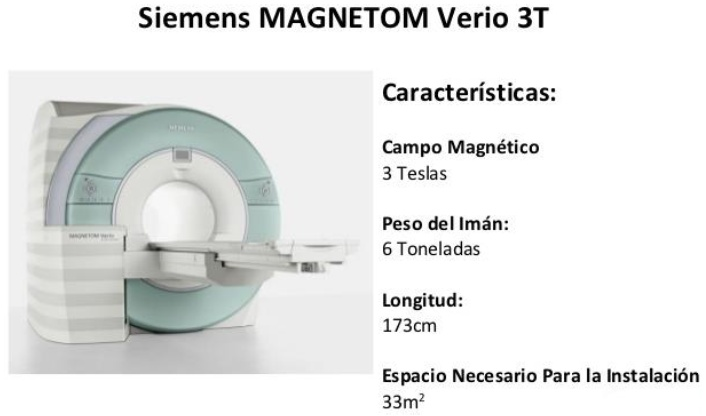
\includegraphics[width=0.9\textwidth]{./Figures/fig443}
	\caption{Equipo comercial de RMN médica}
	\label{fig:443}
\end{figure}
	
	
	\item Aceleradores de partículas: Son equipos que utilizan campos electromagnéticos para acelerar partículas cargadas a altas velocidades. El \textbf{LHC}  \textit{Large Hadron Collider} o gran Colisionador de Hadrones) utiliza materiales superconductores (Niobio y
Titanio a $–271^{o}C$ para generar campos magnéticos intensos y de menor consumo eléctrico.

\begin{figure}[H]
    \centering
    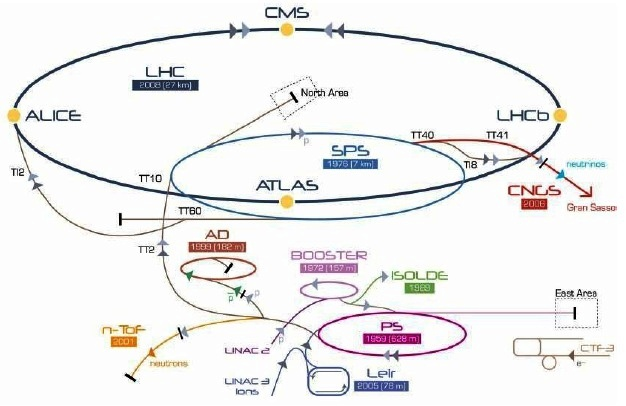
\includegraphics[width=0.9\textwidth]{./Figures/fig444}
	\caption{Concepción esquemática del LHC}
	\label{fig:444}
\end{figure}

	\item Cables superconductores: Téngase en cuenta que entre 10\% y el 15\% de pérdidas se genera en las líneas de transmisión eléctrica. Lograr la disminución es estas sería realmente ventajoso. HTS \textit{High Temperature Superconductor}.
Son cables de transporte eléctrico enfriados con nitrógeno líquido. En la figura se observa el diseño de uno de estos cables. No es de uso frecuente.

\begin{figure}[H]
    \centering
    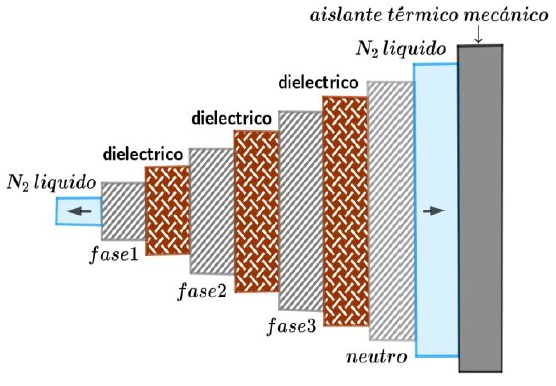
\includegraphics[width=0.7\textwidth]{./Figures/fig445}
	\caption{Cable superconductor}
	\label{fig:445}
\end{figure}


	\item Biomagnetismo: Es el estudio de los campos magnéticos generados por los sistemas biológicos (flujos de corrientes neuronales y fibras musculares). En todas las células de los tejidos biológicos hay un intercambio iónico a través de sus membranas, donde se generan diferencias de potencial eléctricos que llevan asociados campos magnético. La magnitud de estos campos son extremadamente pequeños (entre 50 y 500 $fT$ en el caso de las señales neuro magnéticas). Estas mediciones son realizadas con arreglos de Squid. Presentan importantes ventajas comparativas respecto a las técnicas electroencefalograma (EEG, EMG, etc), ya que no interfieren los tejidos con sus resistencias eléctricas. 
	
\begin{figure}[H]
    \centering
    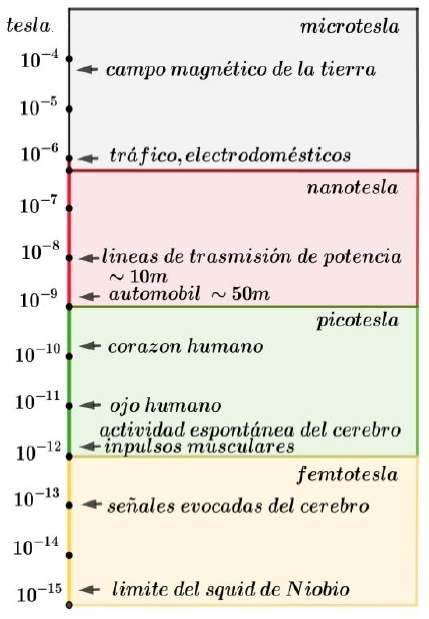
\includegraphics[width=0.6\textwidth]{./Figures/fig446}
	\caption{Órdenes de los distintos campos magnéticos biológicos}
	\label{fig:446}
\end{figure}
	

\end{itemize}


